\def\year{2022}\relax
%File: formatting-instructions-latex-2022.tex
%release 2022.1
\documentclass[letterpaper]{article} % DO NOT CHANGE THIS
\usepackage{aaai22}  % DO NOT CHANGE THIS
\usepackage{times}  % DO NOT CHANGE THIS
\usepackage{helvet}  % DO NOT CHANGE THIS
\usepackage{courier}  % DO NOT CHANGE THIS
\usepackage[hyphens]{url}  % DO NOT CHANGE THIS
\usepackage{longtable}
\usepackage{graphicx} % DO NOT CHANGE THIS
\urlstyle{rm} % DO NOT CHANGE THIS
\def\UrlFont{\rm}  % DO NOT CHANGE THIS
\usepackage{natbib}  % DO NOT CHANGE THIS AND DO NOT ADD ANY OPTIONS TO IT
\usepackage{caption} % DO NOT CHANGE THIS AND DO NOT ADD ANY OPTIONS TO IT
\usepackage{pgf}
\usepackage{pgfplots}
\DeclareCaptionStyle{ruled}{labelfont=normalfont,labelsep=colon,strut=off} % DO NOT CHANGE THIS
\frenchspacing  % DO NOT CHANGE THIS
\setlength{\pdfpagewidth}{8.5in}  % DO NOT CHANGE THIS

\setlength{\pdfpageheight}{11in}  % DO NOT CHANGE THIS
%
% These are recommended to typeset algorithms but not required. See the subsubsection on algorithms. Remove them if you don't have algorithms in your paper.
\usepackage{algorithm}
\usepackage{enumitem}
\usepackage[]{hyperref}
\hypersetup{
    colorlinks=true,
    linkcolor=blue,
    citecolor=blue,
    filecolor=blue,      
    urlcolor=blue,
}


\usetikzlibrary{pgfplots.groupplots}
\usetikzlibrary{shapes.geometric}
\usetikzlibrary{positioning,fit,shapes.geometric,backgrounds, calc}
\usetikzlibrary{arrows,decorations.markings}
\usetikzlibrary{shapes.arrows}
\usetikzlibrary{patterns}
\tikzset{textnode/.style={inner sep=0pt,outer sep=0,execute at begin node={\strut}}}
\tikzstyle{state} = [textnode,circle, draw, inner sep=0pt, outer sep=0]
\usepgfplotslibrary{groupplots}

\pgfplotsset{scaled y ticks=false}
\pgfplotsset{scaled x ticks=false}
                    
\pgfplotsset{every axis/.append style={
                    xlabel={$x$},          % default put x on x-axis
                    ylabel={$y$},          % default put y on y-axis
                    label style={font=\sffamily\small},
                    tick label style={font=\sffamily\small},
                    xticklabel style = {font=\sffamily\scriptsize},
                    title style = {font=\footnotesize\sffamily},
                    ylabel near ticks,
                    y label style={font=\sffamily\scriptsize},
                    xlabel near ticks,
                    x label style={font=\sffamily\scriptsize},
                    legend cell align={left},
                    legend style={draw=none, font=\sffamily\scriptsize},
                    },
                    legend image code/.code={
                    \draw[mark repeat=2,mark phase=2]
                        plot coordinates {
                        (0cm,0cm)
                        (0.15cm,0cm)        %% default is (0.3cm,0cm)
                        (0.3cm,0cm)         %% default is (0.6cm,0cm)
                        };%
                    }
                    }
\pgfplotsset{compat=newest}     


%
% These are are recommended to typeset listings but not required. See the subsubsection on listing. Remove this block if you don't have listings in your paper.
\usepackage{newfloat}
\usepackage{listings}
\lstset{%
	basicstyle={\footnotesize\ttfamily},% footnotesize acceptable for monospace
	numbers=left,numberstyle=\footnotesize,xleftmargin=2em,% show line numbers, remove this entire line if you don't want the numbers.
	aboveskip=0pt,belowskip=0pt,%
	showstringspaces=false,tabsize=2,breaklines=true}
\floatstyle{ruled}
\newfloat{listing}{tb}{lst}{}
\floatname{listing}{Listing}
%
%\nocopyright
%
% PDF Info Is REQUIRED.
% For /Title, write your title in Mixed Case.
% Don't use accents or commands. Retain the parentheses.
% For /Author, add all authors within the parentheses,
% separated by commas. No accents, special characters
% or commands are allowed.
% Keep the /TemplateVersion tag as is
\pdfinfo{
/Title (Truth Social Dataset)
/Author (Anonymous)
}

% DISALLOWED PACKAGES
% \usepackage{authblk} -- This package is specifically forbidden
% \usepackage{balance} -- This package is specifically forbidden
% \usepackage{color (if used in text)
% \usepackage{CJK} -- This package is specifically forbidden
% \usepackage{float} -- This package is specifically forbidden
% \usepackage{flushend} -- This package is specifically forbidden
% \usepackage{fontenc} -- This package is specifically forbidden
% \usepackage{fullpage} -- This package is specifically forbidden
% \usepackage{geometry} -- This package is specifically forbidden
% \usepackage{grffile} -- This package is specifically forbidden
% \usepackage{hyperref} -- This package is specifically forbidden
% \usepackage{navigator} -- This package is specifically forbidden
% (or any other package that embeds links such as navigator or hyperref)
% \indentfirst} -- This package is specifically forbidden
% \layout} -- This package is specifically forbidden
% \multicol} -- This package is specifically forbidden
% \nameref} -- This package is specifically forbidden
% \usepackage{savetrees} -- This package is specifically forbidden
% \usepackage{setspace} -- This package is specifically forbidden
% \usepackage{stfloats} -- This package is specifically forbidden
% \usepackage{tabu} -- This package is specifically forbidden
% \usepackage{titlesec} -- This package is specifically forbidden
% \usepackage{tocbibind} -- This package is specifically forbidden
% \usepackage{ulem} -- This package is specifically forbidden
% \usepackage{wrapfig} -- This package is specifically forbidden
% DISALLOWED COMMANDS
% \nocopyright -- Your paper will not be published if you use this command
% \addtolength -- This command may not be used
% \balance -- This command may not be used
% \baselinestretch -- Your paper will not be published if you use this command
% \clearpage -- No page breaks of any kind may be used for the final version of your paper
% \columnsep -- This command may not be used
% \newpage -- No page breaks of any kind may be used for the final version of your paper
% \pagebreak -- No page breaks of any kind may be used for the final version of your paperr
% \pagestyle -- This command may not be used
% \tiny -- This is not an acceptable font size.
% \vspace{- -- No negative value may be used in proximity of a caption, figure, table, section, subsection, subsubsection, or reference
% \vskip{- -- No negative value may be used to alter spacing above or below a caption, figure, table, section, subsection, subsubsection, or reference
\usepackage{booktabs}

\setcounter{secnumdepth}{0} %May be changed to 1 or 2 if section numbers are desired.


% Title

% Your title must be in mixed case, not sentence case.
% That means all verbs (including short verbs like be, is, using,and go),
% nouns, adverbs, adjectives should be capitalized, including both words in hyphenated terms, while
% articles, conjunctions, and prepositions are lower case unless they
% directly follow a colon or long dash
\title{Truth Social Dataset}
\author{
    %Authors
    % All authors must be in the same font size and format.
    Patrick Gerard, Nicholas Botzer, Tim Weninger
}
\affiliations{
    %Afiliations
    %\textsuperscript{\rm 1}Anonymous Affiliation
    Department of Computer Science and Engineering\\
    University of Notre Dame\\
    Notre Dame, Indiana, USA\\
    \{pgerard2, nbotzer, tweninger\}@nd.edu
    % If you have multiple authors and multiple affiliations
    % use superscripts in text and roman font to identify them.
%
% See more examples next
}


\begin{document}

\maketitle

\begin{abstract}
Formally announced to the public following former President Donald Trump’s bans and suspensions from mainstream social networks in early 2022 after his role in the January 6 Capitol Riots, Truth Social was launched as an ``alternative'' social media platform that claims to be a refuge for free speech, offering a platform for those disaffected by the content moderation policies of the existing, mainstream social networks. The subsequent rise of Truth Social has been driven largely by hard-line supporters of the former president as well as those affected by the content moderation of other social networks. These distinct qualities combined with its status as the main mouthpiece of the former president positions Truth Social as a particularly influential social media platform and give rise to several research questions. However, outside of a handful of news reports, little is known about the new social media platform partially due to a lack of well-curated data. In the current work, we describe a dataset of over 823,000 posts to Truth Social and and social network with over 454,000 distinct users. In addition to the dataset itself, we also present some basic analysis of its content, certain temporal features, and its network.
\end{abstract}


\section{Introduction}
\label{sec:introduction}
The social media platform \textit{Truth Social} was launched in February of 2022 about a year after the suspension of former United States President Donald Trump from Twitter, Facebook, and other social media platforms. Truth Social is largely stylized after Twitter where Tweets are instead called \textit{Truths} and ReTweets are instead called \textit{ReTruths}. Note that throughout the remainder of this paper we most commonly refer to \textit{Truths} as \textit{posts} in order to avoid confusion with the epistemic use of truth (as in true/false). Due to the political and social circumstances surrounding its creation and launch, Truth Social has positioned itself as a hub for right-wing social media users disgruntled by mainstream platforms’ attempts to root out hateful and harmful communities and content.

Since its inception, and largely due to the influence of the former president's use of the platform, Truth Social has increasingly dominated a space of social media platforms that cater to users affiliated with the alt-right political movement---a technology space sometimes referred to as \textit{alt-tech} that also includes Parler, Gab, Rumble and others. Truth Social, in effect, functions as a kind of right-wing Twitter, but without the content regulation that is typically found in mainstream social media platforms. As a result, Truth Social, along with other alt-tech platforms, are a potential hotbed for misinformation, conspiracy theories, and other malign social media activity.


\begin{figure}[t]
\begin{center}
  \includegraphics[width=\linewidth]{figures/my_fillow.png}
  \caption{Annotated illustration of Truth Social Web Interface. The Web scraper extracted user data, and post information, including time, content (with links or other media), quotes, ReTruths, and likes.}
    
\end{center}
\end{figure}

Despite its scope and influence, little is known about the posts and content that is shared on the Truth Social network. The dearth of research involving Truth Social is partially due to how new it is, but also due to the lack of a publically available API. To ameliorate these issues, the current work presents a large dataset of Truths, ReTruths, users, and other data collected from a broad crawl over the Truth Social platform from its launch on February 21, 2022 until October 15, 2022. In total, this dataset contains the content of 823,927 Truths posted by 454,458 users including the full history of the 65,536 most active users. Truth Social does not publish its usage statistics, but we estimate that this dataset contains user data of about 20\% of the total registered users and an unknown, but larger, proportion of the total number of posts.

The dataset represents the first of its kind and can be used to ask and answer numerous research questions. For starters, social media's effects on people's consumption of information has become a topic of increasing importance~\cite{sharot2020people}. Providing users more direct agency over the information they consume, social media---while transformative---may limit exposure to diverse perspectives and cause the formation of like-minded users reinforcing shared narratives~\cite{cinelli2021echo}. This lack of exposure to diverse information and differing perspectives has been found to provide the scaffolding upon which conspiracy theories~\cite{cinelli2022conspiracy} and misinformation~\cite{del2016spreading} may grow. Truth Social is but the latest example of the formation of a self-referential, insular community---commonly called an echo chamber---that  is known to lead to increased political polarization \cite{barbera2020social}. Thus, because Truth Social is itself a right-wing echo chamber, catering to politically polarized defectors of mainstream social media, it provides a fertile ground for the spread of misinformation and conspiracy theories. Therefore, with the increased understanding of conspiracy theories' potentially damaging effects on democracy~\cite{sternisko2020dark}, understanding Truth Social's interaction with echo chambers and misinformation presents an important topic for continued research.


%%Patrick - I feel like these paragraphs repeat themselves, you can tell a singular story with these paragraphs?

% got it


% (notably Twitter~\cite{santucci_2021})
\subsection{A Brief Overview of Truth Social}
Truth Social's announcement and ultimate launch as a social media platform can be traced to former U.S. President Donald Trump's ban from several major social media platforms  following his role in the January 6 United States Capitol attack\footnote{\url{https://blog.twitter.com/en_us/topics/company/2020/suspension}}. As it currently stands, Truth Social is occupied largely by both users disaffected by mainstream platforms’ moderation policies and enthusiastic followers of Donald J. Trump, and appears generally similar to other ``alt-tech" platforms. However, Truth Social's status as the main mouthpiece for a former President whose influence remains momentous in the United States Republican Party positions it as a remarkably influential \textit{alt-tech} platform.

% and current de facto leader of the United States Republican Party positions it as a remarkably influential  ``alt-tech" platform.





% -- launched by a deplatformed former U.S. president and occupied largely by users disaffected by mainstream platforms’ moderation policies -- Truth Social is positioned as a uniquely influential ``alt-tech`` platform.


% POSSIBLE ALT SECOND PARAGRAPH
% Platforms with natures similar to Truth Social -- catering largely to users disaffected by the content moderation of mainstream social networks -- have been found to be decidedly successful in drawing users over from the original platform~\cite{papasavva2021qoincidence}, specifically in the case of followers of Donald Trump~\cite{horta2020does}. Moreover, these types of platform have been shown to both harbor and instigate dangerous conspiracy theories \cite{rye2020reading}. These conspiracy theories, while birthed on seemingly fringe platforms, have been found to ultimately jump to mainstream platforms~\cite{zannettou2017web}, thus advancing the same dangerous misinformation mainstream social networks attempted to thwart via de-platforming~\cite{tollefson2021tracking}.


Platforms with natures similar to Truth Social---catering largely to users disaffected by the content moderation of mainstream social networks---have been found to be decidedly successful in drawing users over from the original platform~\cite{papasavva2021qoincidence}, specifically in the case of followers of Donald Trump~\cite{horta2020does}. Moreover, these types of platforms have been shown to both harbor and instigate dangerous conspiracy theories~\cite{rye2020reading}, which, despite being birthed on seemingly fringe platforms, have been found to ultimately jump to mainstream platforms~\cite{zannettou2017web}, nevertheless advancing the same dangerous misinformation that mainstream social networks attempted to thwart in the first place~\cite{tollefson2021tracking}.



%   OLD
% Truth Social's announcement and ultimate launch as a social media platform can be traced to former U.S. President Donald Trump's ban from several major social media platforms, notably Twitter~\cite{santucci_2021} following his role in the January 6 United States Capitol attack\footnote{\url{https://blog.twitter.com/en_us/topics/company/2020/suspension}}.  Coming after months of allegations of voter fraud in the US presidential election of 2020, the January 6 United States Capitol attack materialized the threat that conspiracy theories may pose to democracy~\cite{sternisko2020dark}. These conspiracy theories of widespread voter fraud (invigorated by Donald Trump's iconic ``Stop the Steal'' campaign~\cite{homans_peterson_2022}) found fertile ground in social media \cite{abilov2021voterfraud2020}; and, despite their lack of credible evidence~\cite{goel2020one}, were shown to have had a significant impact on confidence in election integrity, ultimately permeating throughout the general population and laying the foundation for the January 6 United States Capitol Attack~\cite{berlinski2021effects}. 

% Thus, Truth Social's rise as a social media platform -- launched by a deplatformed former U.S. president and spurred largely by mainstream platforms' attempts to clamp down on misinformation -- positions it as a uniquely influential ``alt-tech'' platform. Platforms with natures similar to Truth Social -- catering largely to users disaffected by the content moderation of mainstream social networks -- have been found to be decidedly successful in drawing users over from the original platform~\cite{papasavva2021qoincidence}, specifically in the case of followers of Donald Trump~\cite{horta2020does}. Moreover, these types of platform have been shown to both harbor and instigate dangerous conspiracy theories \cite{rye2020reading}. These conspiracy theories, while birthed on seemingly fringe platforms, have been found to ultimately jump to mainstream platforms~\cite{zannettou2017web}, thus advancing the same dangerous misinformation mainstream social networks attempted to thwart via de-platforming~\cite{tollefson2021tracking}.





% \section{Overview of TruthSocial}
%Provide background here related to the website itself from a high level so people that haven't heard of it can get a good idea. Also add in some related work on other dataset papers



\section{Dataset Collection Methodology}
%Go over the methodology for how the data was collected here.
%Might want to include that the data is publicly available and we could not find anything prohibiting scraping
\label{sec:dataset_collection}
Collecting the posts and other activity data from Truth Social is not straightforward because the site does not provide a public API. Instead, we implemented a custom Web scraper and programmatically extracted the relevant context from Truth Social's Web interface directly. This Web interface did not impose any crawling restrictions nor did it disallow any crawling with the \texttt{robots.txt} standard. Because no API was available the most straightforward way to collect posts was from each specific account.

We crawled the Truth Social one account at a time, starting with @realDonaldTrump and then iteratively in a breadth first manner over the followers of each account. Specifically, the crawling methodology proceeded as follows:
\begin{enumerate}
  \item Collect information about the user's follower count, following count, creation date.
  \item Iterate through users following the user and users that the user follows, create an edge for each follower-followee relationship, and add that user to the breadth-first queue if that user has not been scraped in the past 14 days.
  \item Extract the full set of available Truths posted by the user.   
\end{enumerate}

This crawl began on September 4, 2022 and continued until October 14, 2022. In that time, all content posted by 65,536 users was collected. The dataset, therefore, has the complete set of all posts for the visited users before September of 2022.

One particular complication of the crawling methodology was the extraction of secondary-posts, \textit{i.e.}, ReTruths, Quotes, and Replies. During the initial crawl, we collected these secondary-posts but not the original post itself. So, at the end of the initial crawl, we additionally collected all of the original posts from which the initially collected ReTruths were based. Due to Truth Social's HTTP request limitations, we were only able to to connect the Quotes and Replies to the user to whom they were directed. Although these efforts resulted in a full accounting of the originating user account for all Quotes and Replies as well as the post content for all ReTruths, the opposite is not true. In other words, although we have the original user for all collected Quotes and Replies and the original post for all collected ReTruths, we we may not have collected all of the ReTruths, Quotes, or Replies for a given post. Nevertheless, as a result of our efforts the dataset is internally consistent.


\subsection{Data Model}

\begin{figure}[t]
    \centering
    \includegraphics[width=\linewidth]{ts_diagram.png}
    \caption{Relationship diagram between data elements in the collected schema. Arrows represent foreign key relationships among the tables.}
    \label{fig:db_diagram}
\end{figure}


During this crawl, data elements were stored in a local database system. The relational schema of this database is illustrated in Fig.~\ref{fig:db_diagram}. This dataset contains various kinds of related data and is therefore modeled as a relational database with foreign key dependencies. For example, follower/followee relationships are enumerated in the \texttt{follows} table, with each entry referencing the following and the followed user via a foreign key to the corresponding \texttt{user} record. Likewise, \texttt{truth} entries are linked to the corresponding \texttt{user}, and  quotes, replies, media, hashtags, external\_urls, and their respective edge tables are all linked with foreign key relationships to further contextualize the content the Truths.


\begin{table}[t]
\centering
\begin{tabular}{ll}
\toprule
Table           & Number of Records \\
\midrule
users.tsv           & 454,458       \\
follows.tsv         & 4,002,115       \\
truths.tsv        & 823,927       \\
quotes.tsv         & 10,508       \\
replies.tsv         & 506,276       \\
media.tsv         & 184,884       \\
hashtags.tsv & 21,599       \\
external\_urls.tsv          & 173,947       \\
truth\_hashtag\_edges.tsv      & 213,295       \\
truth\_media\_edges.tsv         & 257,500       \\
truth\_external\_url\_edges.tsv & 252,877       \\
truth\_user\_tag\_edges.tsv        & 145,234      \\
\end{tabular}
\caption{Description of the Truth Social Dataset}
\label{tab:datapoints}
\end{table}


Tables from the database system were exported to text files in a tab-delimited format and are available on the Zenodo data service at \url{https://doi.org/10.5281/zenodo.7531625} and a sample containing the first 10,000 records from each file are included as Supplemental Material. Table~\ref{tab:datapoints} lists the files available in the dataset and the number of records in each file.




\subsection{FAIR Principles}
The dataset presented by the present work conforms to the FAIR principles~\cite{wilkinson2016fair} and are therefore findable, accessible, interoperable, and re-usable:

\paragraph{Findable:} We provide the dataset publically using the Zenodo data service and give it a permanent digital object identifier (DOI) \url{https://doi.org/10.5281/zenodo.7531625}.
\paragraph{Accessible:} The dataset is freely available on the Internet and can be accessed by anyone with an internet connection. All of the data is provided as tab separated value (TSV) files, a standard format for handling data tabular data. 
\paragraph{Interoperable:} The dataset is easily loaded and viewed with most current database management systems or spreadsheet systems.
\paragraph{Re-usable:} Metadata is also included in a Readme file and is linked to the DOI of this paper for further reference.
    


\subsection{Limitations}
Although we endeavoured to capture a complete and holistic dataset, it is important to be aware of certain methodological and technological limitations and possible sampling biases that may be present in the dataset. Some of the key limitations are are follows:
\begin{enumerate}
    \item \textbf{Access to a user's followers is limited.} While Truth Social permits clients on its Web application to scroll through the entirety of a user's following list, it limits clients' access to a user's followers list to only 50 followers. It is unclear why this limitation exists and how these 50 followers are selected. It may be possible to estimate who follows whom by analyzing a complete following lists of all users and/or the users who frequently ReTruth, Quote or like another user. However, that analysis is not present in the current dataset.
    \item \textbf{Web Request Limits.} Although scraping limits are not published by Truth Social, we did endeavor to be responsible with the number of HTTP requests that were issued to Truth Social. This restricted our ability to capture more data.
    \item \textbf{Sampling Bias.} Recall that the crawling methodology proceeded in a breadth first manner from the a popular user @realDonaldTrump and then proceeded to other highly active users. As a result, this dataset likely contains the most active users of the platform. The choice of @realDonaldTrump as the seed-user may have also nudged the data collection towards more political users and posts. However, the average path length of the user network was relatively small and the post content is quite diverse, so we are confident that the sample is moderately representative of the whole platform.
\end{enumerate}
% \begin{itemize}
%     \item Cannot get all followers.
%     \item BFS structure -- may not have all connections from retruth to truth
%     \item Not all users are accompanied by their respective truths -- created user entries after the fact
% \end{itemize}

\subsection{Ethical Considerations}
The dataset is collected from a publically available resource. Users who submit content do so with the explicit intent of making their activity publically and widely visible. This research was observational only. No intervention or treatment was made to the population; therefore, this research was determined to be exempt from full ethical review panel by the University of Notre Dame institutional review board.


\section{Content Analysis}
To get a better understanding of the collected dataset we performed some rudimentary analysis on the content of the dataset. This analysis includes (1) an investigation into the top-linked Web sites, (2) a look at certain temporal artifacts of the text content of the posts, and (3) an analysis of the follower network of the platform.

\subsection{External Link Analysis}
Research has shown that misinformation campaigns often utilize and share external links to proliferate information across and between multiple platforms~\cite{wilson2020cross, golovchenko2020cross}. For this reason, we extracted the external Web links that users posted. We found 173,947 links in total. The domain of each link was extracted and aggregated for further analysis. 

\begin{figure}[t]
    \centering
    % This file was created with tikzplotlib v0.10.1.
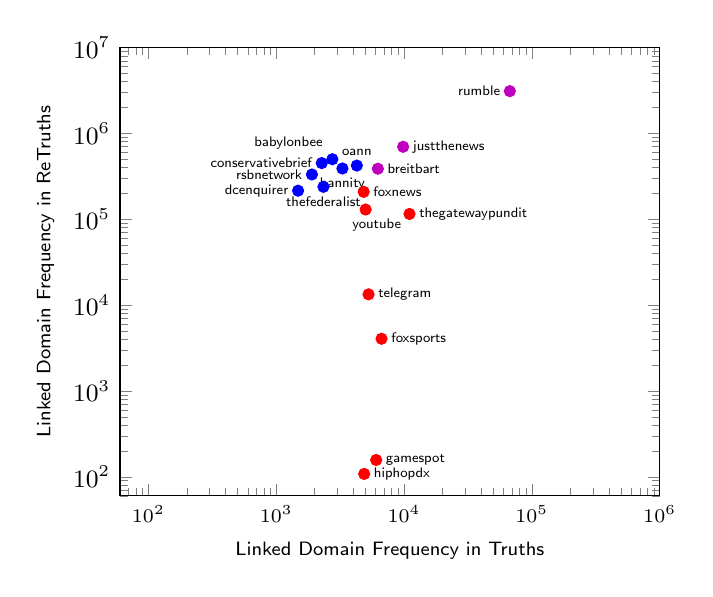
\begin{tikzpicture}

\definecolor{darkgray176}{RGB}{176,176,176}

\begin{axis}[
xlabel={Linked Domain Frequency in Truths},
ylabel={Linked Domain Frequency in ReTruths},
xmode=log, ymode=log,
y grid style={darkgray176},
ymin=60, xmin=60,
ymax=10000000, xmax=1000000,
]
\addplot [
  mark=*,
  only marks,
  scatter,
  nodes near coords,
  scatter/@post marker code/.code={%
  \endscope
},
  scatter/@pre marker code/.code={%
  \expanded{%
  \noexpand\definecolor{thispointdrawcolor}{RGB}{\drawcolor}%
  \noexpand\definecolor{thispointfillcolor}{RGB}{\fillcolor}%
  }%
  \scope[draw=thispointdrawcolor, fill=thispointfillcolor]%
},
  visualization depends on={value \thisrow{draw} \as \drawcolor},
  visualization depends on={value \thisrow{fill} \as \fillcolor}
]
table{%
x  y  draw  fill
67259 3106672 191.25,0,191.25 191.25,0,191.25
9839 698284 191.25,0,191.25 191.25,0,191.25
2750 500040 0,0,255 0,0,255
2272 450811 0,0,255 0,0,255
4274 421838 0,0,255 0,0,255
3297 389997 0,0,255 0,0,255
6244 387704 191.25,0,191.25 191.25,0,191.25
1903 331972 0,0,255 0,0,255
2342 238575 0,0,255 0,0,255
1483 214983 0,0,255 0,0,255
11035 115239 255,0,0 255,0,0
6669 4054 255,0,0 255,0,0
6054 157 255,0,0 255,0,0
5277 13348 255,0,0 255,0,0
5007 129786 255,0,0 255,0,0
4880 108 255,0,0 255,0,0
4837 208491 255,0,0 255,0,0
};
\draw (axis cs:67259,3106672) node[
  font=\sffamily\tiny,
  anchor=east,
  text=black,
  rotate=0.0
]{rumble};
\draw (axis cs:9839,698284) node[
  font=\sffamily\tiny,
  anchor=west,
  text=black,
  rotate=0.0
]{justthenews};
\draw (axis cs:2750,500040) node[
  font=\sffamily\tiny,
  anchor=south east,
  text=black,
  rotate=0.0
]{babylonbee};
\draw (axis cs:2272,450811) node[
  font=\sffamily\tiny,
  anchor=east,
  text=black,
  rotate=0.0
]{conservativebrief};
\draw (axis cs:4274,421838) node[
  font=\sffamily\tiny,
  anchor=south,
  text=black,
  rotate=0.0
]{oann};
\draw (axis cs:3297,389997) node[
  font=\sffamily\tiny,
  anchor=north,
  text=black,
  rotate=0.0
]{hannity};
\draw (axis cs:6244,387704) node[
  font=\sffamily\tiny,
  anchor=west,
  text=black,
  rotate=0.0
]{breitbart};
\draw (axis cs:1903,331972) node[
  font=\sffamily\tiny,
  anchor=east,
  text=black,
  rotate=0.0
]{rsbnetwork};
\draw (axis cs:2342,238575) node[
  font=\sffamily\tiny,
  anchor=north,
  text=black,
  rotate=0.0
]{thefederalist};
\draw (axis cs:1483,214983) node[
  font=\sffamily\tiny,
  anchor=east,
  text=black,
  rotate=0.0
]{dcenquirer};
\draw (axis cs:11035,115239) node[
  font=\sffamily\tiny,
  anchor=west,
  text=black,
  rotate=0.0
]{thegatewaypundit};
\draw (axis cs:6669,4054) node[
  font=\sffamily\tiny,
  anchor=west,
  text=black,
  rotate=0.0
]{foxsports};
\draw (axis cs:6054,157) node[
  font=\sffamily\tiny,
  anchor=west,
  text=black,
  rotate=0.0
]{gamespot};
\draw (axis cs:5277,13348) node[
  font=\sffamily\tiny,
  anchor=west,
  text=black,
  rotate=0.0
]{telegram};
\draw (axis cs:5007,129786) node[
  font=\sffamily\tiny,
  anchor=125,
  text=black,
  rotate=0.0
]{youtube};
\draw (axis cs:4880,108) node[
  font=\sffamily\tiny,
  anchor=west,
  text=black,
  rotate=0.0
]{hiphopdx};
\draw (axis cs:4837,208491) node[
  font=\sffamily\tiny,
  anchor=west,
  text=black,
  rotate=0.0
]{foxnews};
\end{axis}

\end{tikzpicture}

    \caption{Top 10 linked domains appearing in Truths (red, x-axis) and top 10 linked domains appearing in ReTruths (blue, y-axis). Purple marks indicate that the domain is in the top 10 in both Truths and ReTruths.}
    \label{fig:external_links}
\end{figure}

Figure~\ref{fig:external_links} illustrates the top linked domains in terms of the number of Truths in which they appear (x-axis) and the number of ReTruths in which they appear.

% Website with great info on Rumble. https://imge.com/what-is-rumble/
The top linked external Web site in terms of frequency in both Truths and ReTruths is Rumble, a video sharing platform. This site is known for having looser content moderation restrictions compared to many other video sharing platforms like YouTube and has become a haven for controversial figures that have been banned from mainstream platforms. Rumble has grown in popularity in recent years at least partially due to its use by former President Donald Trump to stream his political rallies and post news clips.

Other popular site include right-wing political networks like OANN, Breitbart, FoxNews, etc. Curiously, a large number of external links point to the Telegram social media platform. Popular in Russia, Telegram is frequently used by supporters of Russia in the Russia-Ukraine War~\cite{theisen2023motif}. It has also in been investigated as a platform that acts as a safe haven for those that have been deplatformed from other social media sites~\cite{rogers2020deplatforming}. Because Telegram has this association with deplatformed individuals we further investigated the five most shared telegram channels to better understand the type of content that was shared. In order of decreasing popularity, the five most shared telegram channels are:
\begin{enumerate}
    \item \textbf{RealKarliBonne}. This channel shares a large variety of memes, Truths, and messages supporting Donald Trump. The channel also shares a large amount of video content featuring the Biden administration. Although some video messages are supportive of Trump, the preponderance is negative of the Biden administration and may serve as an example of affective polarization~\cite{iyengar2019origins}.
    \item \textbf{LauraAbolichannel}. This channel does not appear to have a clear focus. Its content contains commentary and clips from right-wing media, anti-vaccination messages, and uplifting memes.
    \item \textbf{freedomforcebattalion}. This channel presents former President Donald Trump's messaging and other current events with a biblical perspective. 
    \item \textbf{realx22report}. This is the official Telegram channel of X22report, a daily show that covers financial and political issues. 
    \item \textbf{drawandstrikechannel} This is the channel of right-wing political columnist Brian Cates. Cates is an active user on Truth Social and draws a major following as well in his Telegram channel. Content in the channel focuses around various political topics and current events.
\end{enumerate}


The combination of Truth Social's politically charged user-base and external links' role in narrative-building and misinformation campaigns creates a significant space for further analysis in both the information contained in the external links and the temporal aspect of the external links.

Examinations into the information contained in the external links may provide major insights into the spread of conspiracy theories and misinformation on Truth Social and across the social Web. For example, to better understand the popularization of conspiracy theories on Truth Social, one may trace the earliest external domains that references a certain conspiracy theory and analyze their role in the narrative spread through Truth Social.


%Examinations into the temporal aspect of external links, \textit{i.e.}, which domains dominate at what point, may provide major insights into the external influences with the greatest effect on Truth Social's users. For example, external links may play a major role in building cohesive narratives around certain events, and further analysis into how narratives jump from external domains to and from Truth Social users is needed to understand how external agents may influence social media users broadly.

Overall, external links in Truth Social remarkably reflect the politically charged user-base, and therefore external agents' influence on the user-base cannot be overlooked. Thus, we believe that further analysis of these external links' role in the Truth Social network is critical to understanding how certain narratives and conspiracy theories propagate across the network.


\begin{figure*}
    \centering
    \pgfplotstableread{
x	y   jan6    jan6like    mar marlike gtrend_j6 gtrend_mar
19024	0.000208725	0	0	0	0	0.05	0.0
19025	0.004383219	0	0	0	0	0.05	0.0
19026	0.014193279	0	0	0	0	0.03	0.0
19027	0.018576498	0	0	0	0	0.04	0.0
19028	0.029221457	0	0	0	0	0.05	0.0
19029	0.016071801	0	0	0	0	0.04	0.01
19030	0.02400334	0	0	0	0	0.03	0.02
19031	0.091838865	0	0	0	0	0.02	0.03
19032	0.126069714	0	0	0	0	0.03	0.02
19033	0.169693175	0	0	0	0	0.03	0.01
19034	0.256522647	0	0	0	0	0.03	0.01
19035	0.257357545	0	0	0	0	0.02	0.01
19036	0.192026717	0	0	0	0	0.02	0.01
19037	0.218326028	0	0	0	0	0.02	0.0
19038	0.490085577	0	0	0	0	0.02	0.01
19039	0.64767272	0	0	0	0	0.02	0.0
19040	0.591525777	0	0	0	0	0.02	0.01
19041	0.554790232	0	0	0	0	0.02	0.01
19042	0.550824463	0	0	0	0	0.02	0.01
19043	0.540388228	0	0	0	0	0.02	0.0
19044	0.426633271	0.002493766	0	0	0	0.01	0.01
19045	0.470048007	0.002493766	0	0.016420361	0.018072289	0.02	0.01
19046	0.673763306	0	0	0	0	0.02	0.0
19047	0.680859946	0	0	0	0	0.02	0.02
19048	0.831141724	0	0	0	0	0.01	0.01
19049	0.894385306	0	0	0.004926108	0.006024096	0.02	0.0
19050	0.923815487	0.002493766	0.005555556	0	0	0.02	0.01
19051	0.906908787	0	0	0	0	0.02	0.01
19052	0.765602171	0	0	0	0	0.02	0.01
19053	0.83719474	0.017456359	0.016666667	0	0	0.03	0.01
19054	0.83719474	0	0	0	0	0.04	0.0
19055	0.834690044	0.017456359	0.011111111	0	0	0.03	0.0
19056	0.888123565	0	0	0	0	0.02	0.0
19057	1	0.042394015	0.038888889	0	0	0.01	0.0
19058	0.623878105	0	0	0	0	0.02	0.0
19059	0.719265289	0.004987531	0.005555556	0	0	0.02	0.0
19060	0.630139846	0	0	0	0	0.02	0.01
19061	0.597161344	0.002493766	0	0	0	0.02	0.02
19062	0.627008975	0.019950125	0.027777778	0.001642036	0	0.02	0.0
19063	0.599248591	0.004987531	0.011111111	0	0	0.01	0.01
19064	0.644541849	0	0	0	0	0.01	0.0
19065	0.478605719	0	0	0	0	0.02	0.0
19066	0.543101649	0	0	0	0	0.02	0.01
19067	0.525151325	0	0	0	0	0.02	0.0
19068	0.49509497	0	0	0	0	0.01	0.02
19069	0.486745982	0	0	0	0	0.02	0.0
19070	0.476309747	0	0	0	0	0.01	0.02
19071	0.486745982	0	0	0	0	0.01	0.0
19072	0.449175537	0	0	0	0	0.02	0.01
19073	0.450219161	0	0	0	0	0.02	0.0
19074	0.407848048	0	0	0	0	0.02	0.0
19075	0.52849092	0	0	0	0	0.02	0.0
19076	0.436443331	0	0	0	0	0.03	0.0
19077	0.418075558	0	0	0	0	0.02	0.0
19078	0.39636819	0.002493766	0	0	0	0.02	0.0
19079	0.361302442	0	0	0	0	0.02	0.0
19080	0.388019203	0.059850374	0.083333333	0	0	0.04	0.0
19081	0.384679608	0.002493766	0	0	0	0.02	0.0
19082	0.424963473	0	0	0	0	0.03	0.02
19083	0.367981632	0	0	0	0	0.02	0.01
19084	0.385931956	0	0	0	0	0.01	0.0
19085	0.319348779	0	0	0	0	0.02	0.01
19086	0.277603841	0.009975062	0.011111111	0	0	0.02	0.01
19087	0.320183678	0	0	0	0	0.02	0.01
19088	0.361928616	0.009975062	0.011111111	0	0	0.02	0.0
19089	0.312460864	0	0	0	0	0.03	0.01
19090	0.307242747	0.012468828	0.016666667	0.001642036	0	0.02	0.01
19091	0.347944062	0	0	0	0	0.01	0.0
19092	0.250052181	0	0	0	0	0.02	0.0
19093	0.256105197	0	0	0	0	0.02	0.0
19094	0.249634732	0	0	0	0	0.02	0.0
19095	0.299102484	0	0	0	0	0.02	0.0
19096	0.280734711	0	0	0	0	0.02	0.0
19097	0.374243373	0.012468828	0.016666667	0	0	0.02	0.0
19098	0.331037362	0	0	0	0	0.01	0.0
19099	0.421415153	0	0	0	0	0.02	0.0
19100	0.426633271	0	0	0	0	0.02	0.0
19101	0.454393655	0.002493766	0	0	0	0.02	0.01
19102	0.458568149	0	0	0	0	0.02	0.01
19103	0.49509497	0.002493766	0	0	0	0.02	0.0
19104	0.574410353	0	0	0	0	0.02	0.0
19105	0.520350657	0	0	0	0	0.02	0.0
19106	0.497599666	0.002493766	0	0	0	0.02	0.0
19107	0.503443957	0	0	0	0	0.02	0.0
19108	0.453976205	0.009975062	0.011111111	0	0	0.02	0.0
19109	0.537257358	0.002493766	0.005555556	0	0	0.02	0.01
19110	0.477144646	0	0	0	0	0.02	0.01
19111	0.443748695	0.002493766	0.005555556	0	0	0.02	0.0
19112	0.455646003	0	0	0.252873563	0.126506024	0.02	0.0
19113	0.374660822	0	0	0	0	0.02	0.0
19114	0.446253392	0	0	0	0	0.02	0.01
19115	0.514506366	0.014962594	0.016666667	0	0	0.02	0.0
19116	0.556460029	0	0	0.027914614	0.018072289	0.01	0.0
19117	0.558338551	0	0	0.003284072	0	0.02	0.02
19118	0.615529117	0	0	0.009852217	0.018072289	0.02	0.01
19119	0.481736589	0.009975062	0.011111111	0	0	0.01	0.01
19120	0.416614485	0.002493766	0	0	0	0.01	0.0
19121	0.459611772	0	0	0	0	0.01	0.0
19122	0.525777499	0	0	0	0	0.02	0.0
19123	0.655812983	0.004987531	0.005555556	0	0	0.02	0.0
19124	0.626174076	0	0	0.001642036	0.006024096	0.02	0.0
19125	0.587351284	0	0	0	0	0.02	0.0
19126	0.690461282	0	0	0	0	0.01	0.0
19127	0.590899603	0	0	0	0	0.01	0.0
19128	0.605510332	0	0	0	0	0.02	0.0
19129	0.677520351	0	0	0	0	0.02	0.0
19130	0.656647881	0	0	0.022988506	0.036144578	0.02	0.0
19131	0.579211021	0	0	0	0	0.02	0.0
19132	0.564391568	0.052369077	0.061111111	0	0	0.02	0.01
19133	0.585681486	0.019950125	0.016666667	0	0	0.01	0.0
19134	0.530995617	0	0	0	0	0.01	0.01
19135	0.544353997	0	0	0	0	0.02	0.0
19136	0.536631183	0.002493766	0	0	0	0.02	0.0
19137	0.628678773	0.002493766	0	0	0	0.02	0.0
19138	0.552076811	0.002493766	0.005555556	0	0	0.01	0.0
19139	0.656021707	0.007481297	0.011111111	0	0	0.01	0.01
19140	0.546441244	0	0	0	0	0.01	0.0
19141	0.554790232	0.02244389	0.022222222	0	0	0.02	0.01
19142	0.672719683	0	0	0	0	0.01	0.0
19143	0.70862033	0.002493766	0	0	0	0.02	0.0
19144	0.602796911	0	0	0	0	0.02	0.0
19145	0.593613024	0	0	0	0	0.02	0.01
19146	0.632435817	0.02244389	0.033333333	0	0	0.02	0.0
19147	0.640367355	0.007481297	0.005555556	0	0	0.02	0.01
19148	0.523064078	0.039900249	0.05	0	0	0.05	0.01
19149	0.452097683	0.037406484	0.033333333	0.004926108	0.006024096	0.08	0.0
19150	0.467125861	0.044887781	0.044444444	0	0	0.11	0.01
19151	0.502400334	0.122194514	0.111111111	0	0	0.11	0.0
19152	0.481527865	1	1	0	0	0.38	0.0
19153	0.429137967	0.074812968	0.061111111	0	0	1.0	0.0
19154	0.425380923	0.072319202	0.055555556	0	0	0.29	0.01
19155	0.420580255	0.281795511	0.183333333	0	0	0.21	0.0
19156	0.368816531	0.049875312	0.044444444	0	0	0.58	0.0
19157	0.404091004	0.034912718	0.027777778	0	0	0.37	0.01
19158	0.445835942	0.024937656	0.016666667	0	0	0.26	0.01
19159	0.44750574	0.004987531	0.005555556	0	0	0.55	0.0
19160	0.484032561	0.037406484	0.027777778	0	0	0.31	0.0
19161	0.587977458	0.019950125	0.011111111	0	0	0.13	0.0
19162	0.35232728	0	0	0	0	0.11	0.01
19163	0.386349405	0.034912718	0.022222222	0	0	0.2	0.01
19164	0.444166145	0.179551122	0.133333333	0	0	0.4	0.0
19165	0.607597579	0.21446384	0.15	0	0	0.23	0.0
19166	0.413901064	0.017456359	0.011111111	0	0	0.51	0.0
19167	0.455019829	0.047381546	0.038888889	0	0	0.17	0.0
19168	0.373408474	0	0	0	0	0.09	0.02
19169	0.362763515	0	0	0	0	0.09	0.0
19170	0.339386349	0.002493766	0	0	0	0.2	0.0
19171	0.35900647	0.476309227	0.311111111	0	0	0.72	0.0
19172	0.348152786	0.014962594	0.011111111	0.001642036	0	0.31	0.0
19173	0.431642663	0.159600998	0.105555556	0	0	0.15	0.01
19174	0.489041954	0.032418953	0.027777778	0	0	0.08	0.01
19175	0.492172824	0.002493766	0	0	0	0.06	0.0
19176	0.399499061	0.127182045	0.066666667	0	0	0.06	0.0
19177	0.376748069	0.259351621	0.155555556	0	0	0.07	0.01
19178	0.415988311	0	0	0	0	0.08	0.0
19179	0.424963473	0.007481297	0.005555556	0	0	0.09	0.0
19180	0.404508453	0	0	0	0	0.08	0.01
19181	0.418910457	0.009975062	0.005555556	0	0	0.09	0.0
19182	0.368399082	0.007481297	0.005555556	0	0	0.06	0.01
19183	0.334168232	0.389027431	0.216666667	0	0	0.09	0.0
19184	0.40033396	0.032418953	0.016666667	0	0	0.17	0.0
19185	0.443748695	0.139650873	0.072222222	0	0	0.52	0.01
19186	0.427468169	0.007481297	0.005555556	0	0	0.21	0.01
19187	0.3727823	0.261845387	0.161111111	0	0	0.16	0.01
19188	0.415362137	0.004987531	0	0	0	0.11	0.0
19189	0.387810478	0	0	0	0	0.07	0.01
19190	0.345856815	0.002493766	0	0	0	0.06	0.02
19191	0.2882488	0.002493766	0	0	0	0.09	0.01
19192	0.346274264	0	0	0	0	0.12	0.01
19193	0.334376957	0.009975062	0.005555556	0	0	0.1	0.0
19194	0.370486329	0.172069825	0.116666667	0	0	0.33	0.0
19195	0.36923398	0.044887781	0.027777778	0	0	0.4	0.01
19196	0.388019203	0.009975062	0.005555556	0	0	0.13	0.0
19197	0.307868921	0.004987531	0.005555556	0	0	0.07	0.0
19198	0.298685034	0.009975062	0.005555556	0	0	0.06	0.0
19199	0.338551451	0.004987531	0.005555556	0	0	0.07	0.0
19200	0.366729284	0.002493766	0	0	0	0.05	0.0
19201	0.429346692	0.002493766	0	0	0	0.04	0.01
19202	0.435817157	0.216957606	0.155555556	0	0	0.03	0.0
19203	0.369860154	0	0	0	0	0.03	0.0
19204	0.304320601	0.117206983	0.072222222	0	0	0.03	0.02
19205	0.3220622	0.004987531	0.005555556	0	0	0.03	0.0
19206	0.608015028	0.164588529	0.105555556	0	0	0.03	0.0
19207	0.58630766	0.009975062	0.005555556	0	0	0.03	0.0
19208	0.55249426	0.019950125	0.011111111	0	0	0.03	0.01
19209	0.608849927	0.007481297	0.011111111	0	0	0.03	0.0
19210	0.477562096	0	0	0	0	0.03	0.0
19211	0.3727823	0.007481297	0.005555556	0	0	0.03	0.01
19212	0.398455437	0	0	0.39408867	0.421686747	0.03	0.27
19213	0.516593613	0.009975062	0.011111111	0.684729064	0.674698795	0.04	1.0
19214	0.550407013	0.007481297	0.005555556	0.881773399	1	0.03	0.44
19215	0.491337925	0.019950125	0.011111111	0.689655172	0.692771084	0.03	0.3
19216	0.456063452	0	0	0.903119869	0.891566265	0.03	0.47
19217	0.455437278	0.027431421	0.022222222	0.167487685	0.180722892	0.02	0.33
19218	0.316635358	0.009975062	0.005555556	0.436781609	0.560240964	0.02	0.22
19219	0.329367564	0	0	1	0.915662651	0.03	0.21
19220	0.471300355	0.002493766	0.005555556	0.742200328	0.668674699	0.03	0.16
19221	0.461699019	0.072319202	0.05	0.201970443	0.222891566	0.03	0.14
19222	0.432060113	0	0	0.348111658	0.36746988	0.02	0.13
19223	0.46128157	0.004987531	0.005555556	0.461412151	0.475903614	0.02	0.1
19224	0.509496973	0	0	0.068965517	0.054216867	0.02	0.1
19225	0.351283657	0.009975062	0.011111111	0.003284072	0.006024096	0.03	0.05
19226	0.337299102	0.002493766	0	0.249589491	0.289156627	0.02	0.07
19227	0.418284283	0.132169576	0.094444444	0.492610837	0.548192771	0.01	0.09
19228	0.532247965	0.002493766	0.005555556	0.266009852	0.246987952	0.02	0.08
19229	0.488833229	0	0	0.203612479	0.186746988	0.02	0.08
19230	0.485702359	0.007481297	0.005555556	0.180623974	0.192771084	0.01	0.27
19231	0.496764767	0.009975062	0.005555556	0.308702791	0.295180723	0.02	0.16
19232	0.414318514	0	0	0.159277504	0.162650602	0.02	0.1
19233	0.373617199	0	0	0.307060755	0.355421687	0.02	0.09
19234	0.487372156	0	0	0.835796388	0.825301205	0.02	0.08
19235	0.461072845	0.019950125	0.011111111	0.249589491	0.246987952	0.02	0.12
19236	0.49154665	0	0	0.026272578	0.030120482	0.03	0.1
19237	0.52890837	0	0	0.036124795	0.042168675	0.04	0.08
19238	0.47818827	0.002493766	0	0.011494253	0.018072289	0.02	0.07
19239	0.327697767	0.002493766	0.005555556	0.077175698	0.072289157	0.02	0.03
19240	0.448966813	0	0	0.085385878	0.078313253	0.03	0.05
19241	0.417031935	0	0	0.285714286	0.289156627	0.03	0.03
19242	0.52181173	0	0	0.234811166	0.28313253	0.03	0.06
19243	0.547067418	0.019950125	0.016666667	0.26272578	0.277108434	0.03	0.06
19244	0.517845961	0	0	0.02955665	0.030120482	0.03	0.03
19245	0.464621165	0	0	0	0	0.02	0.02
19246	0.434982258	0	0	0	0	0.03	0.02
19247	0.31183469	0.007481297	0.005555556	0.052545156	0.072289157	0.03	0.04
19248	0.391984972	0.002493766	0	0.229885057	0.337349398	0.02	0.03
19249	0.378626592	0	0	0.008210181	0.006024096	0.03	0.02
19250	0.398246713	0	0	0.006568144	0.006024096	0.03	0.01
19251	0.470048007	0	0	0.016420361	0.024096386	0.02	0.03
19252	0.427885619	0.024937656	0.027777778	0	0	0.02	0.02
19253	0.315591735	0	0	0.008210181	0.012048193	0.02	0.02
19254	0.376748069	0	0	0.003284072	0.006024096	0.02	0.02
19255	0.423084951	0	0	0.003284072	0.006024096	0.03	0.04
19256	0.349405135	0.004987531	0.005555556	0	0	0.03	0.03
19257	0.273638071	0	0	0.008210181	0.012048193	0.03	0.05
19258	0.35274473	0.004987531	0.005555556	0	0	0.03	0.03
19259	0.398455437	0	0	0	0	0.03	0.04
19260	0.243164266	0	0	0	0	0.04	0.04
19261	0.248591108	0.002493766	0	0.001642036	0	0.07	0.03
19262	0.257148821	0	0	0	0	0.1	0.09
19263	0.299519933	0	0	0	0	0.14	0.25
19264	0.330202463	0	0	0	0	0.07	0.25
19265	0.329576289	0	0	0.001642036	0	0.03	0.12
19266	0.248799833	0	0	0	0	0.02	0.08
19267	0.214986433	0	0	0	0	0.02	0.05
19268	0.166144855	0	0	0	0	0.04	0.02
19269	0.226675016	0	0	0.001642036	0	0.04	0.03
19270	0.250678355	0	0	0	0	0.04	0.04
19271	0.279691087	0	0	0.001642036	0	0.04	0.02
19272	0.227092465	0	0	0	0	0.03	0.01
}{\data}


% This file was created with tikzplotlib v0.10.1.
\begin{tikzpicture}


\begin{axis}[
width=17cm, height=8cm,
xlabel={Date},
xmin=19014.5, xmax=19280.5,
ymin=-0.05, ymax=1.15,
xtick={19024,19052,19083,19113,19144,19174,19205,19236,19266},
xticklabel style={rotate=25.0},
xticklabels={
  Feb 2022,
  Mar 2022,
  Apr 2022,
  May 2022,
  Jun 2022,
  Jul 2022,
  Aug 2022,
  Sep 2022,
  Oct 2022
},
ylabel={Max-Normalized Frequency},
%ymin=-250.1, ymax=5252.1,
ytick style={color=black},
legend pos=north east
]



\addplot +[black, solid, mark=none] table [x=x, y=y] {\data};


\addplot +[blue!50!black, solid, mark=none] table [x=x, y=jan6] {\data};
%\addplot +[teal!50!black, dashed, mark=none] table [x=x, y=jan6like] {\data};

\addplot +[red!50!black, solid, mark=none] table [x=x, y=mar] {\data};
%\addplot +[orange!50!black, dashed, mark=none] table [x=x, y=marlike] {\data};

\addplot +[black, dashed, mark=none] coordinates
{(19044, 0) (19044, 1)} node[above, rotate=0, font=\tiny] {Truth Social Official Launch};
\addplot +[blue, dashed, mark=none] coordinates
{(19152, 0) (19152, 1)} node[text width=2cm, align=center, above, rotate=0, font=\tiny] {January 6 Committee\\Public Hearings Begin};
\addplot +[red, dashed, mark=none] coordinates
{(19212, 0) (19212, 1)} node[above, rotate=0, font=\tiny] {FBI Search of Mar-a-Lago};

%\addplot +[orange!50!black, solid, mark=none]
%table{};
\addplot +[blue, dotted, mark=none] table [x=x, y=gtrend_j6] {\data};


\addplot +[red, dotted, mark=none] table [x=x, y=gtrend_mar] {\data};




% you can see me being dumb in real-time



\legend{Total, Jan 6 Truths, FBI Truths,,,,}%Jan 6 Google Searches, FBI Google Searches}




\end{axis}

\end{tikzpicture}

    \caption{Daily max-normalized frequency of Truths posted in the dataset. Because Truth Social has a strong affiliation with former United States President Donald Trump, political activity and news stories involving the former president are commonly discussed on the site. In this figure, posts mentioning political events like the US House of Representative's Special Committee on the January 6 riots at the US Capitol (blue) and the FBI search at the former president's residence (Mar-a-Lago) spike surrounding these events. Dotted blue and red lines illustrate the data from Google Trends corresponding to the event.}
    \label{fig:daily_truth}
\end{figure*}

\subsection{Text Analysis}
To better understand both the temporal nature of the dataset and the possible interaction between external events and popular topics on Truth Social, we next performed a text analysis on the 823,927 posts in the dataset.


Figure~\ref{fig:daily_truth} provides an example illustration of our findings. Max-normalized by posts per day, the frequency of all posts provides a backdrop for our further evaluation into posts containing certain keywords. Overall, we found that the daily frequency of posts was highest near the official launch of Truth Social, before falling slightly and stabilizing.

Because of its affiliation with the former president, posts on Truth Social largely revolve around activities related to conservative politics and news stories. To illustrate this more concretely we considered two events that occurred during dates covered by the data collection methodology involving the former president: (1) the public hearings from the United States' House of Representative's Select Committee on the January 6 riots at the Capitol Building, and (2) the FBI raid of the former president's residence commonly called Mar-a-Lago.

Our first text analysis centers on the January 6 United States Capitol attack. Utilizing the keywords ``January 6'', ``January Six'', ``Jan 6'', and ``Jan Six'', we identified posts containing any of these phrases (with case-insensitive criteria). As shown in solid blue in Fig.~\ref{fig:daily_truth}, immediately following the start of the January 6 Committee's Public Hearings, posts containing these phrases spiked and continued to be elevated for approximately ten weeks. We believe that further evaluation may find correlation between these repetitive spikes and the ensuing broadcasts of the January 6 Committee's public hearings, but a thorough analysis is outside the scope of the current paper.

Next, we analyzed posts related to the FBI raid of Mar-a-Lago, utilizing the keywords ``Mar-a-Lago'' and ``Mar a Lago''. Illustrated in solid red in Fig.~\ref{fig:daily_truth}, we again identified posts containing any of these phrases (with case-insensitive criteria). Like in the January 6 example above, in this case we also found that Truths containing these phrases spiked following the events.

Dotted blue and red lines in Fig.~\ref{fig:daily_truth} illustrate the data from Google Trends for the January 6 and Mar-a-Lago searches, respectively. We see that the attention of these two events are symmetrical across Truth Social and the Web in general. This symmetry shows that the topics discussed on Truth Social appears to be largely representative of activity on the Web. 

When evaluating these spikes, we found that they were often driven largely by a small number of original posts that were ReTruthed many times. Some of the most popular posts originated from the former president himself, 
but were elevated and expanded by popular commentators, whose roles in narrative-building on Truth Social is a clear topic for further inspection. For example, following the FBI search of Mar-a-Lago, the former president posted ``A horrible thing that took place yesterday at Mar-a-Lago. We are no better than a third world country, a banana republic. It is a continuation of Russia, Russia, Russia, Impeachment Hoax \#1, Impeachment Hoax \# 2, the no collusion Mueller Report, and more. To make matters worse it is all, in my opinion, a coordinated attack with Radical Left Democrat state and local D.A.'s and A.G.'s''. This set off a conspiracy-laden narrative of the events that echoed throughout the platform. These posts typically gathered tens of thousands of ReTruths and likes---a large number for the relatively small platform. These findings and the dataset as a whole may provide much needed insight into the cohesion of the Truth Social platform as well as a better understanding of the role that popular commentators play in driving the narrative for the majority of users.

Ultimately, external events appear to have significant influence on Truth Social's user network. Moreover, the near-immediate rise in posts following certain events may point to both the interests of users and the cohesiveness of the Truth Social network. Further work lies in both the examination of narratives and sentiments accompanying apparent reactions to external events, as well as the examination of the platform-wide influence of a small group of popular commentators and if the narratives and stories that percolate within Truth Social eventually make their way onto mainstream social media platforms.

\subsection{Network Analysis}
Like Facebook, Instagram, and Twitter, the friendship network (via followers or ReTruths) of the Truth Social platform forms a social network that can be analyzed to find social roles, and network-based artifacts like centrality, betweeness, cliques, and other interesting network-based phenomena. 


Because the follower graph could not be reliably extracted from the Web interface, we instead used ReTruths to construct the network. Although not the same as the follower graph, ReTweets (the Twitter-analog to ReTruths) are known to ``more closely mirror real-world relationships and trust''~\cite{bild2015aggregate}. 

\begin{figure}
    \centering
    \input{figures/follower_graph}
    \caption{Degree distribution of the ReTruth graph by distinct users (left) and by total number of ReTruths (right). The red circle represents @realDonaldTrump who has the most ReTruths according to both criteria.}
    \label{fig:graph}
\end{figure}

We used two different criteria to analyze the network. First, we found the number of unique, fully-scraped users who ReTruthed a user. Figure~\ref{fig:graph} (left) illustrates the degree distribution of the ReTruth graph, that is, the number of distinct users who Retruthed another user. This distribution appeared to follow the generally followed typical power-law degree distribution found on Twitter. The user with the highest number of distinct ReTruthing users was ReTruthed by 1,448 users.

Rather than looking at distinct users, our next analysis looked at the total number of ReTruths for each user. Figure~\ref{fig:graph} (right) shows that the ReTruth multi-graph, where multiple ReTruths from the same user count as multiple edges, has a slightly different degree distribution that more closely resembles a log-normal distribution. The user with the highest number of  ReTruths was ReTruthed 1,0176,833 times.



%\begin{figure}
%    \centering
%    \pgfplotstableread{
x	px
0	0.8522186279296875
1	0.00506591796875
2	0.004974365234375
3	0.0038604736328125
4	0.0038299560546875
5	0.0036468505859375
6	0.0030364990234375
7	0.0028076171875
8	0.002838134765625
9	0.0022430419921875
10	0.00225830078125
11	0.0020751953125
12	0.00201416015625
13	0.0017852783203125
14	0.0017547607421875
15	0.001312255859375
16	0.0013275146484375
17	0.0012664794921875
18	0.0013275146484375
19	0.00146484375
20	0.0012664794921875
21	0.001190185546875
22	0.00103759765625
23	0.0009002685546875
24	0.0008087158203125
25	0.001129150390625
26	0.00103759765625
27	0.00067138671875
28	0.0010223388671875
29	0.0007476806640625
30	0.0008392333984375
31	0.0008544921875
32	0.000762939453125
33	0.0010833740234375
34	0.000701904296875
35	0.0005950927734375
36	0.0007171630859375
37	0.00054931640625
38	0.0005340576171875
39	0.00054931640625
40	0.000579833984375
41	0.000579833984375
42	0.000518798828125
43	0.0005340576171875
44	0.000579833984375
45	0.0005950927734375
46	0.00054931640625
47	0.0005950927734375
48	0.0004119873046875
49	0.0005035400390625
50	0.00048828125
51	0.000518798828125
52	0.000518798828125
53	0.000518798828125
54	0.00042724609375
55	0.0004119873046875
56	0.0005035400390625
57	0.000457763671875
58	0.0003204345703125
59	0.0004119873046875
60	0.0003814697265625
61	0.000335693359375
62	0.0003662109375
63	0.0003814697265625
64	0.000335693359375
65	0.0003509521484375
66	0.00030517578125
67	0.0003662109375
68	0.000335693359375
69	0.0003662109375
70	0.0002899169921875
71	0.0002899169921875
72	0.000213623046875
73	0.0002593994140625
74	0.000335693359375
75	0.0002899169921875
76	0.00030517578125
77	0.000274658203125
78	0.000274658203125
79	0.0003509521484375
80	0.000213623046875
81	0.00030517578125
82	0.0003204345703125
83	0.00030517578125
84	0.0001678466796875
85	0.000213623046875
86	0.000335693359375
87	0.00018310546875
88	0.000274658203125
89	0.0001983642578125
90	0.000335693359375
91	0.000244140625
92	0.0002288818359375
93	0.00018310546875
94	0.0001220703125
95	0.0001678466796875
96	0.00018310546875
97	0.0001678466796875
98	0.0001373291015625
99	0.0002593994140625
100	0.000213623046875
101	0.0002288818359375
102	0.000274658203125
103	0.000213623046875
104	0.00030517578125
105	0.0001983642578125
106	0.0001678466796875
107	0.00018310546875
108	0.0002288818359375
109	0.0001983642578125
110	0.0001983642578125
111	0.0001678466796875
112	0.00018310546875
113	0.000152587890625
114	0.000274658203125
115	0.0001678466796875
116	0.0001220703125
117	0.00018310546875
118	0.0001678466796875
119	0.000213623046875
120	0.00018310546875
121	0.0001220703125
122	0.000152587890625
123	0.00018310546875
124	0.0001373291015625
125	0.000152587890625
126	7.62939453125e-05
127	0.0001373291015625
128	0.0001220703125
129	0.0002288818359375
130	0.00018310546875
131	0.0001373291015625
132	0.0001983642578125
133	0.0001220703125
134	0.000213623046875
135	0.0001220703125
136	0.0001373291015625
137	0.0001068115234375
138	0.0002593994140625
139	0.000152587890625
140	0.0001220703125
141	0.000213623046875
142	0.0001220703125
143	0.000152587890625
144	0.0001220703125
145	9.1552734375e-05
146	0.0001373291015625
147	0.00018310546875
148	0.0001373291015625
149	0.0001373291015625
150	0.0001373291015625
151	0.00018310546875
152	0.0001220703125
153	0.0001983642578125
154	0.000152587890625
155	0.0001373291015625
156	6.103515625e-05
157	0.0001373291015625
158	0.000152587890625
159	6.103515625e-05
160	6.103515625e-05
161	0.00018310546875
162	6.103515625e-05
163	0.0001068115234375
164	0.0001220703125
165	0.0001373291015625
166	4.57763671875e-05
167	0.000152587890625
168	0.0001220703125
169	0.000152587890625
170	0.000152587890625
171	4.57763671875e-05
172	0.0001068115234375
173	9.1552734375e-05
174	0.0001220703125
175	0.000152587890625
176	0.00018310546875
177	3.0517578125e-05
178	9.1552734375e-05
179	7.62939453125e-05
180	0.00018310546875
181	6.103515625e-05
182	0.0001068115234375
183	0.0001220703125
184	0.0001220703125
185	9.1552734375e-05
186	0.0001220703125
187	0.0001068115234375
188	9.1552734375e-05
189	0.0001220703125
190	0.0001373291015625
191	0.00018310546875
192	0.0001220703125
193	9.1552734375e-05
194	7.62939453125e-05
195	9.1552734375e-05
196	0.0001220703125
197	0.000152587890625
198	0.0001068115234375
199	7.62939453125e-05
200	9.1552734375e-05
201	0.0001678466796875
202	7.62939453125e-05
203	6.103515625e-05
204	4.57763671875e-05
205	4.57763671875e-05
206	0.0001373291015625
207	6.103515625e-05
208	9.1552734375e-05
209	0.000152587890625
210	9.1552734375e-05
211	4.57763671875e-05
212	3.0517578125e-05
213	7.62939453125e-05
214	4.57763671875e-05
215	0.0001678466796875
216	9.1552734375e-05
217	0.0001220703125
218	7.62939453125e-05
219	9.1552734375e-05
220	0.0001068115234375
221	3.0517578125e-05
222	0.0001068115234375
223	0.0001220703125
224	6.103515625e-05
225	0.0001068115234375
226	4.57763671875e-05
227	9.1552734375e-05
228	9.1552734375e-05
229	9.1552734375e-05
230	3.0517578125e-05
231	4.57763671875e-05
232	0.0001373291015625
233	7.62939453125e-05
234	7.62939453125e-05
235	0.000152587890625
236	9.1552734375e-05
237	0.0001068115234375
238	9.1552734375e-05
239	6.103515625e-05
240	0.0001220703125
241	0.0001220703125
242	0.0001220703125
243	4.57763671875e-05
244	0.0001068115234375
245	0.0001068115234375
246	0.0001068115234375
247	4.57763671875e-05
248	6.103515625e-05
249	0.0001068115234375
250	4.57763671875e-05
251	0.0001220703125
252	0.0001068115234375
253	6.103515625e-05
254	7.62939453125e-05
255	4.57763671875e-05
256	6.103515625e-05
257	0.0001068115234375
258	1.52587890625e-05
259	6.103515625e-05
260	3.0517578125e-05
261	9.1552734375e-05
262	7.62939453125e-05
263	0.0001068115234375
264	9.1552734375e-05
265	7.62939453125e-05
266	4.57763671875e-05
267	4.57763671875e-05
268	4.57763671875e-05
269	4.57763671875e-05
270	6.103515625e-05
271	6.103515625e-05
272	0.000152587890625
273	4.57763671875e-05
274	6.103515625e-05
275	0.0001220703125
276	4.57763671875e-05
277	0.0001220703125
278	6.103515625e-05
279	7.62939453125e-05
280	6.103515625e-05
281	6.103515625e-05
282	4.57763671875e-05
283	7.62939453125e-05
284	7.62939453125e-05
285	0.0001068115234375
286	7.62939453125e-05
287	7.62939453125e-05
288	3.0517578125e-05
289	3.0517578125e-05
290	6.103515625e-05
291	4.57763671875e-05
292	6.103515625e-05
293	4.57763671875e-05
294	0.0001220703125
295	6.103515625e-05
296	1.52587890625e-05
297	6.103515625e-05
298	4.57763671875e-05
299	6.103515625e-05
300	3.0517578125e-05
301	0.000152587890625
302	0.0001373291015625
303	7.62939453125e-05
304	0.0001220703125
305	6.103515625e-05
306	3.0517578125e-05
307	0.0001068115234375
308	4.57763671875e-05
309	6.103515625e-05
310	0.0001068115234375
311	4.57763671875e-05
312	6.103515625e-05
313	1.52587890625e-05
314	4.57763671875e-05
315	6.103515625e-05
316	4.57763671875e-05
317	6.103515625e-05
318	3.0517578125e-05
319	9.1552734375e-05
320	6.103515625e-05
321	3.0517578125e-05
322	9.1552734375e-05
323	3.0517578125e-05
324	7.62939453125e-05
325	3.0517578125e-05
326	4.57763671875e-05
328	1.52587890625e-05
329	3.0517578125e-05
330	4.57763671875e-05
331	9.1552734375e-05
332	4.57763671875e-05
333	1.52587890625e-05
334	7.62939453125e-05
335	4.57763671875e-05
336	3.0517578125e-05
337	4.57763671875e-05
338	1.52587890625e-05
339	3.0517578125e-05
340	4.57763671875e-05
341	7.62939453125e-05
342	4.57763671875e-05
343	9.1552734375e-05
344	9.1552734375e-05
345	3.0517578125e-05
346	9.1552734375e-05
347	4.57763671875e-05
348	0.0001068115234375
349	7.62939453125e-05
350	4.57763671875e-05
351	9.1552734375e-05
352	3.0517578125e-05
353	4.57763671875e-05
354	6.103515625e-05
355	4.57763671875e-05
356	3.0517578125e-05
357	1.52587890625e-05
358	7.62939453125e-05
360	1.52587890625e-05
361	6.103515625e-05
362	6.103515625e-05
363	3.0517578125e-05
364	7.62939453125e-05
365	6.103515625e-05
366	4.57763671875e-05
367	3.0517578125e-05
368	3.0517578125e-05
369	7.62939453125e-05
370	6.103515625e-05
371	4.57763671875e-05
372	3.0517578125e-05
373	6.103515625e-05
374	7.62939453125e-05
375	3.0517578125e-05
376	3.0517578125e-05
377	3.0517578125e-05
378	7.62939453125e-05
379	7.62939453125e-05
380	4.57763671875e-05
381	7.62939453125e-05
382	7.62939453125e-05
383	3.0517578125e-05
384	6.103515625e-05
385	1.52587890625e-05
386	4.57763671875e-05
387	7.62939453125e-05
389	1.52587890625e-05
390	3.0517578125e-05
391	3.0517578125e-05
392	3.0517578125e-05
393	3.0517578125e-05
394	6.103515625e-05
395	1.52587890625e-05
396	1.52587890625e-05
398	3.0517578125e-05
399	3.0517578125e-05
400	4.57763671875e-05
401	3.0517578125e-05
402	7.62939453125e-05
403	3.0517578125e-05
404	3.0517578125e-05
405	4.57763671875e-05
406	1.52587890625e-05
407	3.0517578125e-05
408	1.52587890625e-05
409	4.57763671875e-05
410	4.57763671875e-05
411	1.52587890625e-05
412	3.0517578125e-05
413	4.57763671875e-05
415	1.52587890625e-05
416	1.52587890625e-05
417	3.0517578125e-05
418	3.0517578125e-05
419	4.57763671875e-05
420	3.0517578125e-05
421	1.52587890625e-05
422	3.0517578125e-05
423	3.0517578125e-05
424	6.103515625e-05
426	4.57763671875e-05
427	3.0517578125e-05
428	4.57763671875e-05
430	6.103515625e-05
431	1.52587890625e-05
432	4.57763671875e-05
434	0.0001068115234375
435	1.52587890625e-05
436	4.57763671875e-05
438	4.57763671875e-05
439	3.0517578125e-05
440	1.52587890625e-05
442	9.1552734375e-05
443	6.103515625e-05
445	1.52587890625e-05
446	0.0001068115234375
447	1.52587890625e-05
448	7.62939453125e-05
449	3.0517578125e-05
450	4.57763671875e-05
451	7.62939453125e-05
453	4.57763671875e-05
454	1.52587890625e-05
455	4.57763671875e-05
456	4.57763671875e-05
457	3.0517578125e-05
458	3.0517578125e-05
459	3.0517578125e-05
460	3.0517578125e-05
461	6.103515625e-05
462	6.103515625e-05
463	4.57763671875e-05
464	6.103515625e-05
465	1.52587890625e-05
466	6.103515625e-05
467	1.52587890625e-05
468	6.103515625e-05
469	4.57763671875e-05
470	1.52587890625e-05
471	9.1552734375e-05
472	4.57763671875e-05
473	1.52587890625e-05
474	6.103515625e-05
475	3.0517578125e-05
476	3.0517578125e-05
477	1.52587890625e-05
478	1.52587890625e-05
479	3.0517578125e-05
480	4.57763671875e-05
481	4.57763671875e-05
482	1.52587890625e-05
483	6.103515625e-05
485	6.103515625e-05
486	3.0517578125e-05
487	4.57763671875e-05
488	9.1552734375e-05
489	4.57763671875e-05
490	4.57763671875e-05
491	1.52587890625e-05
492	1.52587890625e-05
493	1.52587890625e-05
495	3.0517578125e-05
496	1.52587890625e-05
497	3.0517578125e-05
498	9.1552734375e-05
499	4.57763671875e-05
500	3.0517578125e-05
502	3.0517578125e-05
503	1.52587890625e-05
504	3.0517578125e-05
506	3.0517578125e-05
507	1.52587890625e-05
508	7.62939453125e-05
510	4.57763671875e-05
511	1.52587890625e-05
512	1.52587890625e-05
513	4.57763671875e-05
514	3.0517578125e-05
515	1.52587890625e-05
516	1.52587890625e-05
517	3.0517578125e-05
518	1.52587890625e-05
521	3.0517578125e-05
522	1.52587890625e-05
523	1.52587890625e-05
524	1.52587890625e-05
525	4.57763671875e-05
527	4.57763671875e-05
529	6.103515625e-05
530	4.57763671875e-05
531	6.103515625e-05
532	1.52587890625e-05
533	7.62939453125e-05
534	1.52587890625e-05
535	3.0517578125e-05
536	3.0517578125e-05
537	1.52587890625e-05
538	1.52587890625e-05
539	4.57763671875e-05
540	1.52587890625e-05
541	4.57763671875e-05
542	1.52587890625e-05
543	3.0517578125e-05
544	9.1552734375e-05
545	1.52587890625e-05
546	3.0517578125e-05
547	4.57763671875e-05
548	1.52587890625e-05
549	1.52587890625e-05
550	1.52587890625e-05
551	6.103515625e-05
552	1.52587890625e-05
553	1.52587890625e-05
554	1.52587890625e-05
555	4.57763671875e-05
556	1.52587890625e-05
557	6.103515625e-05
559	4.57763671875e-05
560	6.103515625e-05
561	6.103515625e-05
562	1.52587890625e-05
563	1.52587890625e-05
564	1.52587890625e-05
565	1.52587890625e-05
566	3.0517578125e-05
567	3.0517578125e-05
568	1.52587890625e-05
569	4.57763671875e-05
570	3.0517578125e-05
571	3.0517578125e-05
572	4.57763671875e-05
573	3.0517578125e-05
574	1.52587890625e-05
575	3.0517578125e-05
576	3.0517578125e-05
577	1.52587890625e-05
578	3.0517578125e-05
579	1.52587890625e-05
582	1.52587890625e-05
584	1.52587890625e-05
585	3.0517578125e-05
586	1.52587890625e-05
587	1.52587890625e-05
588	1.52587890625e-05
589	4.57763671875e-05
590	3.0517578125e-05
591	7.62939453125e-05
592	3.0517578125e-05
594	6.103515625e-05
595	7.62939453125e-05
596	3.0517578125e-05
598	1.52587890625e-05
599	1.52587890625e-05
600	1.52587890625e-05
601	3.0517578125e-05
602	1.52587890625e-05
603	4.57763671875e-05
604	1.52587890625e-05
605	3.0517578125e-05
606	1.52587890625e-05
607	9.1552734375e-05
609	1.52587890625e-05
610	1.52587890625e-05
612	3.0517578125e-05
613	4.57763671875e-05
614	1.52587890625e-05
615	3.0517578125e-05
617	1.52587890625e-05
618	1.52587890625e-05
619	3.0517578125e-05
620	1.52587890625e-05
622	3.0517578125e-05
624	3.0517578125e-05
625	3.0517578125e-05
627	6.103515625e-05
630	3.0517578125e-05
631	1.52587890625e-05
632	4.57763671875e-05
633	1.52587890625e-05
634	3.0517578125e-05
635	3.0517578125e-05
637	3.0517578125e-05
639	1.52587890625e-05
642	4.57763671875e-05
643	3.0517578125e-05
644	3.0517578125e-05
645	4.57763671875e-05
646	4.57763671875e-05
647	1.52587890625e-05
648	6.103515625e-05
650	3.0517578125e-05
653	3.0517578125e-05
654	4.57763671875e-05
655	3.0517578125e-05
658	1.52587890625e-05
659	1.52587890625e-05
660	3.0517578125e-05
661	1.52587890625e-05
662	3.0517578125e-05
663	3.0517578125e-05
664	6.103515625e-05
665	1.52587890625e-05
666	3.0517578125e-05
667	1.52587890625e-05
669	4.57763671875e-05
670	1.52587890625e-05
671	3.0517578125e-05
672	1.52587890625e-05
673	1.52587890625e-05
674	1.52587890625e-05
675	3.0517578125e-05
677	1.52587890625e-05
678	1.52587890625e-05
679	3.0517578125e-05
680	3.0517578125e-05
681	1.52587890625e-05
682	1.52587890625e-05
683	1.52587890625e-05
684	1.52587890625e-05
685	6.103515625e-05
686	4.57763671875e-05
688	1.52587890625e-05
689	1.52587890625e-05
690	3.0517578125e-05
691	1.52587890625e-05
692	1.52587890625e-05
694	3.0517578125e-05
695	1.52587890625e-05
696	3.0517578125e-05
698	3.0517578125e-05
701	1.52587890625e-05
703	1.52587890625e-05
707	4.57763671875e-05
709	1.52587890625e-05
711	3.0517578125e-05
713	1.52587890625e-05
714	1.52587890625e-05
716	1.52587890625e-05
718	3.0517578125e-05
719	1.52587890625e-05
720	4.57763671875e-05
721	3.0517578125e-05
722	3.0517578125e-05
723	3.0517578125e-05
725	6.103515625e-05
726	1.52587890625e-05
727	4.57763671875e-05
728	1.52587890625e-05
729	1.52587890625e-05
730	4.57763671875e-05
731	1.52587890625e-05
732	1.52587890625e-05
733	1.52587890625e-05
735	4.57763671875e-05
736	1.52587890625e-05
737	1.52587890625e-05
738	1.52587890625e-05
740	3.0517578125e-05
741	1.52587890625e-05
742	1.52587890625e-05
743	1.52587890625e-05
744	1.52587890625e-05
745	1.52587890625e-05
746	3.0517578125e-05
747	1.52587890625e-05
748	1.52587890625e-05
750	3.0517578125e-05
751	1.52587890625e-05
753	6.103515625e-05
755	1.52587890625e-05
757	3.0517578125e-05
758	1.52587890625e-05
760	6.103515625e-05
761	1.52587890625e-05
762	3.0517578125e-05
763	3.0517578125e-05
764	1.52587890625e-05
765	3.0517578125e-05
766	4.57763671875e-05
768	3.0517578125e-05
769	1.52587890625e-05
770	1.52587890625e-05
771	3.0517578125e-05
773	3.0517578125e-05
774	3.0517578125e-05
777	6.103515625e-05
778	1.52587890625e-05
779	1.52587890625e-05
780	3.0517578125e-05
781	1.52587890625e-05
782	1.52587890625e-05
783	1.52587890625e-05
784	1.52587890625e-05
785	1.52587890625e-05
787	1.52587890625e-05
790	1.52587890625e-05
791	1.52587890625e-05
792	1.52587890625e-05
793	1.52587890625e-05
794	1.52587890625e-05
795	1.52587890625e-05
797	3.0517578125e-05
798	1.52587890625e-05
799	1.52587890625e-05
803	1.52587890625e-05
804	3.0517578125e-05
806	6.103515625e-05
807	1.52587890625e-05
809	3.0517578125e-05
810	3.0517578125e-05
812	1.52587890625e-05
813	1.52587890625e-05
815	1.52587890625e-05
817	3.0517578125e-05
822	1.52587890625e-05
825	1.52587890625e-05
827	1.52587890625e-05
828	1.52587890625e-05
829	1.52587890625e-05
830	1.52587890625e-05
832	1.52587890625e-05
836	3.0517578125e-05
839	1.52587890625e-05
840	1.52587890625e-05
842	1.52587890625e-05
843	1.52587890625e-05
845	3.0517578125e-05
846	1.52587890625e-05
851	3.0517578125e-05
852	1.52587890625e-05
853	1.52587890625e-05
854	1.52587890625e-05
855	1.52587890625e-05
859	4.57763671875e-05
860	1.52587890625e-05
861	4.57763671875e-05
865	1.52587890625e-05
866	3.0517578125e-05
867	1.52587890625e-05
871	1.52587890625e-05
874	1.52587890625e-05
876	1.52587890625e-05
877	1.52587890625e-05
878	4.57763671875e-05
879	1.52587890625e-05
880	1.52587890625e-05
882	1.52587890625e-05
885	1.52587890625e-05
886	1.52587890625e-05
887	1.52587890625e-05
888	4.57763671875e-05
890	1.52587890625e-05
892	4.57763671875e-05
894	4.57763671875e-05
895	1.52587890625e-05
897	1.52587890625e-05
899	1.52587890625e-05
902	6.103515625e-05
903	1.52587890625e-05
905	1.52587890625e-05
906	1.52587890625e-05
907	3.0517578125e-05
910	3.0517578125e-05
912	4.57763671875e-05
913	4.57763671875e-05
917	1.52587890625e-05
920	3.0517578125e-05
921	3.0517578125e-05
923	1.52587890625e-05
924	3.0517578125e-05
926	4.57763671875e-05
928	3.0517578125e-05
930	1.52587890625e-05
933	3.0517578125e-05
935	1.52587890625e-05
936	3.0517578125e-05
938	1.52587890625e-05
941	3.0517578125e-05
943	1.52587890625e-05
944	1.52587890625e-05
945	1.52587890625e-05
946	1.52587890625e-05
949	1.52587890625e-05
952	1.52587890625e-05
953	1.52587890625e-05
958	3.0517578125e-05
960	1.52587890625e-05
961	1.52587890625e-05
962	1.52587890625e-05
971	1.52587890625e-05
972	1.52587890625e-05
974	3.0517578125e-05
975	1.52587890625e-05
978	1.52587890625e-05
979	1.52587890625e-05
980	3.0517578125e-05
981	1.52587890625e-05
982	3.0517578125e-05
983	3.0517578125e-05
984	3.0517578125e-05
989	1.52587890625e-05
990	1.52587890625e-05
991	1.52587890625e-05
993	1.52587890625e-05
995	1.52587890625e-05
996	3.0517578125e-05
999	1.52587890625e-05
1000	7.62939453125e-05
1003	1.52587890625e-05
1004	1.52587890625e-05
1006	1.52587890625e-05
1007	1.52587890625e-05
1008	1.52587890625e-05
1009	1.52587890625e-05
1010	1.52587890625e-05
1011	3.0517578125e-05
1012	1.52587890625e-05
1014	3.0517578125e-05
1015	1.52587890625e-05
1016	3.0517578125e-05
1017	4.57763671875e-05
1018	3.0517578125e-05
1019	1.52587890625e-05
1020	3.0517578125e-05
1024	3.0517578125e-05
1026	1.52587890625e-05
1028	3.0517578125e-05
1030	1.52587890625e-05
1031	3.0517578125e-05
1033	3.0517578125e-05
1038	3.0517578125e-05
1040	6.103515625e-05
1041	1.52587890625e-05
1044	3.0517578125e-05
1046	3.0517578125e-05
1047	4.57763671875e-05
1049	1.52587890625e-05
1050	1.52587890625e-05
1051	1.52587890625e-05
1053	1.52587890625e-05
1058	1.52587890625e-05
1060	4.57763671875e-05
1061	1.52587890625e-05
1062	1.52587890625e-05
1063	1.52587890625e-05
1066	1.52587890625e-05
1068	1.52587890625e-05
1071	1.52587890625e-05
1076	1.52587890625e-05
1079	1.52587890625e-05
1085	3.0517578125e-05
1086	1.52587890625e-05
1087	1.52587890625e-05
1090	3.0517578125e-05
1093	4.57763671875e-05
1096	1.52587890625e-05
1097	1.52587890625e-05
1100	3.0517578125e-05
1101	1.52587890625e-05
1111	1.52587890625e-05
1115	1.52587890625e-05
1116	1.52587890625e-05
1117	1.52587890625e-05
1119	1.52587890625e-05
1120	3.0517578125e-05
1121	1.52587890625e-05
1122	1.52587890625e-05
1127	3.0517578125e-05
1128	1.52587890625e-05
1130	1.52587890625e-05
1135	1.52587890625e-05
1144	1.52587890625e-05
1147	3.0517578125e-05
1150	1.52587890625e-05
1152	1.52587890625e-05
1153	3.0517578125e-05
1156	1.52587890625e-05
1160	3.0517578125e-05
1161	1.52587890625e-05
1162	1.52587890625e-05
1163	1.52587890625e-05
1167	1.52587890625e-05
1168	3.0517578125e-05
1169	3.0517578125e-05
1170	1.52587890625e-05
1173	4.57763671875e-05
1174	3.0517578125e-05
1176	1.52587890625e-05
1177	1.52587890625e-05
1178	1.52587890625e-05
1179	6.103515625e-05
1182	3.0517578125e-05
1190	3.0517578125e-05
1191	1.52587890625e-05
1192	3.0517578125e-05
1193	1.52587890625e-05
1195	1.52587890625e-05
1199	1.52587890625e-05
1200	1.52587890625e-05
1204	1.52587890625e-05
1205	4.57763671875e-05
1213	4.57763671875e-05
1216	1.52587890625e-05
1218	1.52587890625e-05
1219	1.52587890625e-05
1220	1.52587890625e-05
1222	1.52587890625e-05
1223	1.52587890625e-05
1224	1.52587890625e-05
1225	1.52587890625e-05
1226	4.57763671875e-05
1228	1.52587890625e-05
1229	3.0517578125e-05
1230	3.0517578125e-05
1232	1.52587890625e-05
1233	1.52587890625e-05
1235	1.52587890625e-05
1237	3.0517578125e-05
1239	3.0517578125e-05
1240	3.0517578125e-05
1246	1.52587890625e-05
1247	1.52587890625e-05
1250	3.0517578125e-05
1253	1.52587890625e-05
1256	1.52587890625e-05
1257	1.52587890625e-05
1260	1.52587890625e-05
1269	1.52587890625e-05
1270	4.57763671875e-05
1272	3.0517578125e-05
1277	3.0517578125e-05
1283	1.52587890625e-05
1284	3.0517578125e-05
1285	1.52587890625e-05
1295	1.52587890625e-05
1298	1.52587890625e-05
1299	3.0517578125e-05
1301	1.52587890625e-05
1302	1.52587890625e-05
1304	1.52587890625e-05
1305	3.0517578125e-05
1306	1.52587890625e-05
1308	1.52587890625e-05
1310	1.52587890625e-05
1313	1.52587890625e-05
1316	3.0517578125e-05
1320	1.52587890625e-05
1322	1.52587890625e-05
1326	1.52587890625e-05
1329	1.52587890625e-05
1330	1.52587890625e-05
1336	1.52587890625e-05
1337	1.52587890625e-05
1342	1.52587890625e-05
1345	1.52587890625e-05
1348	1.52587890625e-05
1355	3.0517578125e-05
1363	3.0517578125e-05
1364	1.52587890625e-05
1367	4.57763671875e-05
1370	1.52587890625e-05
1371	1.52587890625e-05
1374	1.52587890625e-05
1376	1.52587890625e-05
1377	1.52587890625e-05
1380	1.52587890625e-05
1387	1.52587890625e-05
1390	3.0517578125e-05
1391	1.52587890625e-05
1392	3.0517578125e-05
1393	1.52587890625e-05
1394	1.52587890625e-05
1395	1.52587890625e-05
1397	3.0517578125e-05
1400	1.52587890625e-05
1402	1.52587890625e-05
1403	3.0517578125e-05
1405	1.52587890625e-05
1410	4.57763671875e-05
1415	3.0517578125e-05
1419	1.52587890625e-05
1430	3.0517578125e-05
1438	3.0517578125e-05
1439	1.52587890625e-05
1441	1.52587890625e-05
1447	1.52587890625e-05
1450	1.52587890625e-05
1454	1.52587890625e-05
1460	6.103515625e-05
1471	3.0517578125e-05
1473	1.52587890625e-05
1474	1.52587890625e-05
1475	1.52587890625e-05
1477	1.52587890625e-05
1479	1.52587890625e-05
1485	1.52587890625e-05
1486	1.52587890625e-05
1489	1.52587890625e-05
1491	1.52587890625e-05
1496	1.52587890625e-05
1498	1.52587890625e-05
1501	1.52587890625e-05
1503	1.52587890625e-05
1504	1.52587890625e-05
1506	1.52587890625e-05
1509	3.0517578125e-05
1511	1.52587890625e-05
1517	1.52587890625e-05
1519	1.52587890625e-05
1520	1.52587890625e-05
1522	1.52587890625e-05
1526	3.0517578125e-05
1527	1.52587890625e-05
1529	1.52587890625e-05
1531	1.52587890625e-05
1533	1.52587890625e-05
1534	1.52587890625e-05
1538	1.52587890625e-05
1541	1.52587890625e-05
1547	1.52587890625e-05
1548	3.0517578125e-05
1550	1.52587890625e-05
1552	3.0517578125e-05
1560	1.52587890625e-05
1564	3.0517578125e-05
1566	3.0517578125e-05
1568	3.0517578125e-05
1569	1.52587890625e-05
1572	1.52587890625e-05
1581	3.0517578125e-05
1583	1.52587890625e-05
1585	1.52587890625e-05
1591	1.52587890625e-05
1596	1.52587890625e-05
1597	1.52587890625e-05
1600	1.52587890625e-05
1601	3.0517578125e-05
1603	1.52587890625e-05
1609	1.52587890625e-05
1614	1.52587890625e-05
1617	1.52587890625e-05
1620	1.52587890625e-05
1630	3.0517578125e-05
1634	1.52587890625e-05
1637	1.52587890625e-05
1638	1.52587890625e-05
1640	1.52587890625e-05
1649	3.0517578125e-05
1650	1.52587890625e-05
1653	1.52587890625e-05
1655	1.52587890625e-05
1658	1.52587890625e-05
1660	4.57763671875e-05
1661	1.52587890625e-05
1662	1.52587890625e-05
1668	1.52587890625e-05
1671	3.0517578125e-05
1672	1.52587890625e-05
1674	1.52587890625e-05
1679	1.52587890625e-05
1681	1.52587890625e-05
1682	1.52587890625e-05
1683	1.52587890625e-05
1689	1.52587890625e-05
1691	3.0517578125e-05
1692	1.52587890625e-05
1694	1.52587890625e-05
1698	3.0517578125e-05
1700	1.52587890625e-05
1701	1.52587890625e-05
1711	1.52587890625e-05
1712	1.52587890625e-05
1713	1.52587890625e-05
1716	1.52587890625e-05
1719	1.52587890625e-05
1727	1.52587890625e-05
1729	1.52587890625e-05
1732	3.0517578125e-05
1738	1.52587890625e-05
1740	1.52587890625e-05
1741	1.52587890625e-05
1742	1.52587890625e-05
1746	1.52587890625e-05
1748	1.52587890625e-05
1750	1.52587890625e-05
1751	1.52587890625e-05
1755	1.52587890625e-05
1760	1.52587890625e-05
1763	3.0517578125e-05
1770	1.52587890625e-05
1774	1.52587890625e-05
1777	1.52587890625e-05
1783	1.52587890625e-05
1785	1.52587890625e-05
1786	1.52587890625e-05
1790	3.0517578125e-05
1797	1.52587890625e-05
1799	1.52587890625e-05
1800	3.0517578125e-05
1806	1.52587890625e-05
1810	1.52587890625e-05
1811	1.52587890625e-05
1816	1.52587890625e-05
1821	1.52587890625e-05
1824	1.52587890625e-05
1825	1.52587890625e-05
1832	3.0517578125e-05
1833	1.52587890625e-05
1836	3.0517578125e-05
1845	1.52587890625e-05
1847	3.0517578125e-05
1848	3.0517578125e-05
1850	3.0517578125e-05
1853	1.52587890625e-05
1855	1.52587890625e-05
1856	1.52587890625e-05
1857	1.52587890625e-05
1858	1.52587890625e-05
1865	1.52587890625e-05
1868	1.52587890625e-05
1870	1.52587890625e-05
1873	3.0517578125e-05
1874	1.52587890625e-05
1877	1.52587890625e-05
1878	1.52587890625e-05
1879	1.52587890625e-05
1883	1.52587890625e-05
1891	1.52587890625e-05
1893	1.52587890625e-05
1894	1.52587890625e-05
1896	1.52587890625e-05
1897	1.52587890625e-05
1903	1.52587890625e-05
1910	3.0517578125e-05
1914	1.52587890625e-05
1916	1.52587890625e-05
1917	1.52587890625e-05
1918	1.52587890625e-05
1924	1.52587890625e-05
1930	1.52587890625e-05
1932	1.52587890625e-05
1937	1.52587890625e-05
1939	1.52587890625e-05
1940	3.0517578125e-05
1941	1.52587890625e-05
1947	1.52587890625e-05
1948	1.52587890625e-05
1951	1.52587890625e-05
1952	3.0517578125e-05
1953	1.52587890625e-05
1956	1.52587890625e-05
1957	1.52587890625e-05
1958	1.52587890625e-05
1962	1.52587890625e-05
1963	1.52587890625e-05
1965	1.52587890625e-05
1967	1.52587890625e-05
1972	1.52587890625e-05
1979	1.52587890625e-05
1987	1.52587890625e-05
1989	1.52587890625e-05
2002	1.52587890625e-05
2008	3.0517578125e-05
2011	1.52587890625e-05
2019	3.0517578125e-05
2020	1.52587890625e-05
2029	1.52587890625e-05
2030	1.52587890625e-05
2032	1.52587890625e-05
2033	1.52587890625e-05
2041	3.0517578125e-05
2042	1.52587890625e-05
2043	1.52587890625e-05
2052	1.52587890625e-05
2063	1.52587890625e-05
2070	3.0517578125e-05
2071	1.52587890625e-05
2077	1.52587890625e-05
2079	1.52587890625e-05
2085	3.0517578125e-05
2088	1.52587890625e-05
2090	1.52587890625e-05
2100	1.52587890625e-05
2101	1.52587890625e-05
2102	1.52587890625e-05
2105	1.52587890625e-05
2106	1.52587890625e-05
2107	1.52587890625e-05
2109	1.52587890625e-05
2115	1.52587890625e-05
2143	1.52587890625e-05
2152	1.52587890625e-05
2157	1.52587890625e-05
2160	1.52587890625e-05
2173	1.52587890625e-05
2175	1.52587890625e-05
2176	1.52587890625e-05
2178	1.52587890625e-05
2188	1.52587890625e-05
2199	1.52587890625e-05
2203	1.52587890625e-05
2204	1.52587890625e-05
2214	1.52587890625e-05
2218	1.52587890625e-05
2225	1.52587890625e-05
2227	1.52587890625e-05
2238	1.52587890625e-05
2239	1.52587890625e-05
2241	1.52587890625e-05
2261	1.52587890625e-05
2265	1.52587890625e-05
2272	3.0517578125e-05
2276	1.52587890625e-05
2280	1.52587890625e-05
2281	1.52587890625e-05
2286	3.0517578125e-05
2287	1.52587890625e-05
2290	1.52587890625e-05
2293	1.52587890625e-05
2301	1.52587890625e-05
2304	1.52587890625e-05
2306	1.52587890625e-05
2316	1.52587890625e-05
2326	1.52587890625e-05
2333	1.52587890625e-05
2338	1.52587890625e-05
2340	3.0517578125e-05
2346	1.52587890625e-05
2347	1.52587890625e-05
2360	1.52587890625e-05
2361	1.52587890625e-05
2365	1.52587890625e-05
2368	1.52587890625e-05
2370	1.52587890625e-05
2371	1.52587890625e-05
2376	3.0517578125e-05
2378	1.52587890625e-05
2381	1.52587890625e-05
2386	1.52587890625e-05
2388	3.0517578125e-05
2391	1.52587890625e-05
2393	3.0517578125e-05
2396	1.52587890625e-05
2404	3.0517578125e-05
2406	1.52587890625e-05
2409	1.52587890625e-05
2410	1.52587890625e-05
2414	1.52587890625e-05
2421	1.52587890625e-05
2424	1.52587890625e-05
2435	1.52587890625e-05
2440	1.52587890625e-05
2458	1.52587890625e-05
2460	1.52587890625e-05
2463	1.52587890625e-05
2467	1.52587890625e-05
2479	1.52587890625e-05
2481	1.52587890625e-05
2483	1.52587890625e-05
2489	1.52587890625e-05
2497	3.0517578125e-05
2501	1.52587890625e-05
2511	1.52587890625e-05
2515	1.52587890625e-05
2520	1.52587890625e-05
2527	1.52587890625e-05
2532	1.52587890625e-05
2535	1.52587890625e-05
2546	1.52587890625e-05
2571	1.52587890625e-05
2580	1.52587890625e-05
2581	1.52587890625e-05
2588	1.52587890625e-05
2599	1.52587890625e-05
2608	1.52587890625e-05
2611	1.52587890625e-05
2622	1.52587890625e-05
2624	1.52587890625e-05
2629	1.52587890625e-05
2630	1.52587890625e-05
2633	1.52587890625e-05
2635	1.52587890625e-05
2638	3.0517578125e-05
2647	1.52587890625e-05
2650	1.52587890625e-05
2651	3.0517578125e-05
2657	1.52587890625e-05
2659	1.52587890625e-05
2663	1.52587890625e-05
2665	1.52587890625e-05
2679	1.52587890625e-05
2680	1.52587890625e-05
2688	1.52587890625e-05
2689	1.52587890625e-05
2692	1.52587890625e-05
2695	1.52587890625e-05
2699	1.52587890625e-05
2703	1.52587890625e-05
2704	1.52587890625e-05
2709	1.52587890625e-05
2712	1.52587890625e-05
2720	1.52587890625e-05
2721	1.52587890625e-05
2722	1.52587890625e-05
2728	1.52587890625e-05
2729	1.52587890625e-05
2735	1.52587890625e-05
2751	1.52587890625e-05
2766	1.52587890625e-05
2768	3.0517578125e-05
2770	1.52587890625e-05
2774	1.52587890625e-05
2777	1.52587890625e-05
2797	1.52587890625e-05
2799	1.52587890625e-05
2804	1.52587890625e-05
2813	1.52587890625e-05
2815	1.52587890625e-05
2823	1.52587890625e-05
2844	1.52587890625e-05
2845	1.52587890625e-05
2855	1.52587890625e-05
2857	1.52587890625e-05
2860	1.52587890625e-05
2868	1.52587890625e-05
2870	1.52587890625e-05
2884	1.52587890625e-05
2887	1.52587890625e-05
2889	3.0517578125e-05
2899	1.52587890625e-05
2904	1.52587890625e-05
2907	1.52587890625e-05
2915	1.52587890625e-05
2926	1.52587890625e-05
2931	1.52587890625e-05
2934	1.52587890625e-05
2945	1.52587890625e-05
2948	1.52587890625e-05
2953	3.0517578125e-05
2956	1.52587890625e-05
2959	1.52587890625e-05
2966	1.52587890625e-05
2971	1.52587890625e-05
2977	1.52587890625e-05
2993	1.52587890625e-05
3001	1.52587890625e-05
3021	1.52587890625e-05
3027	1.52587890625e-05
3033	1.52587890625e-05
3034	1.52587890625e-05
3043	1.52587890625e-05
3066	1.52587890625e-05
3077	1.52587890625e-05
3078	1.52587890625e-05
3083	1.52587890625e-05
3093	1.52587890625e-05
3097	1.52587890625e-05
3105	1.52587890625e-05
3108	1.52587890625e-05
3110	1.52587890625e-05
3119	3.0517578125e-05
3120	1.52587890625e-05
3127	1.52587890625e-05
3128	1.52587890625e-05
3130	1.52587890625e-05
3133	1.52587890625e-05
3134	1.52587890625e-05
3146	1.52587890625e-05
3161	1.52587890625e-05
3167	1.52587890625e-05
3174	1.52587890625e-05
3175	1.52587890625e-05
3180	1.52587890625e-05
3186	1.52587890625e-05
3198	1.52587890625e-05
3207	1.52587890625e-05
3209	1.52587890625e-05
3221	3.0517578125e-05
3225	1.52587890625e-05
3254	1.52587890625e-05
3262	1.52587890625e-05
3267	1.52587890625e-05
3272	1.52587890625e-05
3279	1.52587890625e-05
3280	1.52587890625e-05
3283	1.52587890625e-05
3284	1.52587890625e-05
3287	1.52587890625e-05
3296	1.52587890625e-05
3298	1.52587890625e-05
3320	1.52587890625e-05
3325	1.52587890625e-05
3328	1.52587890625e-05
3335	1.52587890625e-05
3338	1.52587890625e-05
3339	1.52587890625e-05
3358	1.52587890625e-05
3369	1.52587890625e-05
3375	1.52587890625e-05
3391	1.52587890625e-05
3397	1.52587890625e-05
3402	1.52587890625e-05
3409	3.0517578125e-05
3430	1.52587890625e-05
3435	1.52587890625e-05
3442	1.52587890625e-05
3447	1.52587890625e-05
3451	1.52587890625e-05
3476	3.0517578125e-05
3479	1.52587890625e-05
3510	1.52587890625e-05
3526	1.52587890625e-05
3530	1.52587890625e-05
3541	1.52587890625e-05
3542	1.52587890625e-05
3546	1.52587890625e-05
3553	1.52587890625e-05
3554	1.52587890625e-05
3574	1.52587890625e-05
3580	1.52587890625e-05
3582	1.52587890625e-05
3596	1.52587890625e-05
3598	1.52587890625e-05
3601	1.52587890625e-05
3605	1.52587890625e-05
3611	1.52587890625e-05
3623	1.52587890625e-05
3630	1.52587890625e-05
3633	1.52587890625e-05
3638	1.52587890625e-05
3650	1.52587890625e-05
3665	1.52587890625e-05
3682	1.52587890625e-05
3696	1.52587890625e-05
3697	1.52587890625e-05
3706	1.52587890625e-05
3707	1.52587890625e-05
3719	1.52587890625e-05
3723	3.0517578125e-05
3734	1.52587890625e-05
3735	1.52587890625e-05
3741	1.52587890625e-05
3744	1.52587890625e-05
3764	1.52587890625e-05
3789	1.52587890625e-05
3804	1.52587890625e-05
3808	1.52587890625e-05
3829	1.52587890625e-05
3842	1.52587890625e-05
3848	1.52587890625e-05
3856	1.52587890625e-05
3869	1.52587890625e-05
3876	1.52587890625e-05
3899	1.52587890625e-05
3914	1.52587890625e-05
3919	1.52587890625e-05
3922	3.0517578125e-05
3923	3.0517578125e-05
3924	1.52587890625e-05
3950	1.52587890625e-05
3960	1.52587890625e-05
3964	1.52587890625e-05
3981	1.52587890625e-05
3989	1.52587890625e-05
3994	1.52587890625e-05
4027	1.52587890625e-05
4029	1.52587890625e-05
4030	1.52587890625e-05
4031	1.52587890625e-05
4040	1.52587890625e-05
4042	1.52587890625e-05
4052	1.52587890625e-05
4061	1.52587890625e-05
4070	1.52587890625e-05
4101	1.52587890625e-05
4105	1.52587890625e-05
4117	1.52587890625e-05
4124	1.52587890625e-05
4132	3.0517578125e-05
4142	1.52587890625e-05
4185	1.52587890625e-05
4186	3.0517578125e-05
4193	1.52587890625e-05
4209	1.52587890625e-05
4217	1.52587890625e-05
4219	1.52587890625e-05
4223	1.52587890625e-05
4224	1.52587890625e-05
4228	1.52587890625e-05
4234	1.52587890625e-05
4238	1.52587890625e-05
4247	1.52587890625e-05
4253	1.52587890625e-05
4273	1.52587890625e-05
4304	1.52587890625e-05
4309	1.52587890625e-05
4317	1.52587890625e-05
4320	1.52587890625e-05
4331	1.52587890625e-05
4343	1.52587890625e-05
4385	1.52587890625e-05
4387	1.52587890625e-05
4403	1.52587890625e-05
4405	1.52587890625e-05
4406	1.52587890625e-05
4410	1.52587890625e-05
4413	1.52587890625e-05
4423	1.52587890625e-05
4479	1.52587890625e-05
4480	1.52587890625e-05
4562	1.52587890625e-05
4582	1.52587890625e-05
4597	1.52587890625e-05
4614	1.52587890625e-05
4620	3.0517578125e-05
4624	1.52587890625e-05
4648	1.52587890625e-05
4675	1.52587890625e-05
4685	1.52587890625e-05
4695	3.0517578125e-05
4710	1.52587890625e-05
4725	1.52587890625e-05
4761	1.52587890625e-05
4766	1.52587890625e-05
4775	1.52587890625e-05
4780	1.52587890625e-05
4796	1.52587890625e-05
4811	1.52587890625e-05
4817	1.52587890625e-05
4828	1.52587890625e-05
4832	1.52587890625e-05
4854	1.52587890625e-05
4860	1.52587890625e-05
4894	1.52587890625e-05
4899	1.52587890625e-05
4918	1.52587890625e-05
4924	1.52587890625e-05
4925	1.52587890625e-05
4936	1.52587890625e-05
4940	1.52587890625e-05
4958	1.52587890625e-05
4960	1.52587890625e-05
4961	1.52587890625e-05
5007	1.52587890625e-05
5023	1.52587890625e-05
5026	1.52587890625e-05
5048	1.52587890625e-05
5058	1.52587890625e-05
5082	1.52587890625e-05
5099	1.52587890625e-05
5172	1.52587890625e-05
5213	1.52587890625e-05
5219	1.52587890625e-05
5228	1.52587890625e-05
5250	1.52587890625e-05
5255	1.52587890625e-05
5267	1.52587890625e-05
5272	1.52587890625e-05
5299	1.52587890625e-05
5304	1.52587890625e-05
5305	1.52587890625e-05
5308	1.52587890625e-05
5357	1.52587890625e-05
5373	1.52587890625e-05
5379	1.52587890625e-05
5381	1.52587890625e-05
5395	1.52587890625e-05
5396	1.52587890625e-05
5402	1.52587890625e-05
5408	1.52587890625e-05
5416	1.52587890625e-05
5418	1.52587890625e-05
5476	1.52587890625e-05
5491	1.52587890625e-05
5509	1.52587890625e-05
5511	1.52587890625e-05
5513	1.52587890625e-05
5521	1.52587890625e-05
5547	1.52587890625e-05
5555	1.52587890625e-05
5567	1.52587890625e-05
5589	1.52587890625e-05
5611	1.52587890625e-05
5676	1.52587890625e-05
5681	3.0517578125e-05
5687	1.52587890625e-05
5690	1.52587890625e-05
5696	1.52587890625e-05
5714	1.52587890625e-05
5724	1.52587890625e-05
5725	1.52587890625e-05
5731	1.52587890625e-05
5748	1.52587890625e-05
5768	1.52587890625e-05
5809	1.52587890625e-05
5814	1.52587890625e-05
5818	1.52587890625e-05
5826	1.52587890625e-05
5867	1.52587890625e-05
6070	1.52587890625e-05
6072	1.52587890625e-05
6094	1.52587890625e-05
6097	1.52587890625e-05
6111	1.52587890625e-05
6132	1.52587890625e-05
6148	1.52587890625e-05
6201	1.52587890625e-05
6229	1.52587890625e-05
6272	1.52587890625e-05
6273	1.52587890625e-05
6331	1.52587890625e-05
6346	1.52587890625e-05
6355	1.52587890625e-05
6422	1.52587890625e-05
6470	1.52587890625e-05
6505	1.52587890625e-05
6519	1.52587890625e-05
6562	1.52587890625e-05
6579	1.52587890625e-05
6583	1.52587890625e-05
6595	1.52587890625e-05
6596	1.52587890625e-05
6633	1.52587890625e-05
6781	1.52587890625e-05
6786	1.52587890625e-05
6798	1.52587890625e-05
6846	1.52587890625e-05
6871	1.52587890625e-05
6903	1.52587890625e-05
6904	1.52587890625e-05
6905	1.52587890625e-05
6927	1.52587890625e-05
6950	1.52587890625e-05
6983	1.52587890625e-05
6985	1.52587890625e-05
7024	1.52587890625e-05
7031	1.52587890625e-05
7032	1.52587890625e-05
7045	1.52587890625e-05
7059	1.52587890625e-05
7077	1.52587890625e-05
7087	1.52587890625e-05
7101	1.52587890625e-05
7103	1.52587890625e-05
7115	1.52587890625e-05
7207	1.52587890625e-05
7216	1.52587890625e-05
7274	1.52587890625e-05
7297	1.52587890625e-05
7298	1.52587890625e-05
7376	1.52587890625e-05
7395	1.52587890625e-05
7425	3.0517578125e-05
7430	1.52587890625e-05
7447	1.52587890625e-05
7477	1.52587890625e-05
7536	1.52587890625e-05
7597	1.52587890625e-05
7604	1.52587890625e-05
7645	1.52587890625e-05
7691	1.52587890625e-05
7707	1.52587890625e-05
7772	1.52587890625e-05
7774	1.52587890625e-05
7789	1.52587890625e-05
7797	1.52587890625e-05
7804	1.52587890625e-05
7835	1.52587890625e-05
7851	1.52587890625e-05
7882	1.52587890625e-05
7928	1.52587890625e-05
7933	1.52587890625e-05
7967	1.52587890625e-05
7974	1.52587890625e-05
7979	1.52587890625e-05
8034	1.52587890625e-05
8184	1.52587890625e-05
8186	1.52587890625e-05
8233	1.52587890625e-05
8289	1.52587890625e-05
8296	1.52587890625e-05
8353	1.52587890625e-05
8363	1.52587890625e-05
8471	1.52587890625e-05
8481	1.52587890625e-05
8531	1.52587890625e-05
8540	1.52587890625e-05
8560	1.52587890625e-05
8598	1.52587890625e-05
8610	1.52587890625e-05
8759	1.52587890625e-05
8780	1.52587890625e-05
8782	1.52587890625e-05
8788	1.52587890625e-05
8834	1.52587890625e-05
8884	1.52587890625e-05
8910	1.52587890625e-05
8936	1.52587890625e-05
8976	1.52587890625e-05
9072	1.52587890625e-05
9092	1.52587890625e-05
9143	1.52587890625e-05
9149	1.52587890625e-05
9162	1.52587890625e-05
9164	1.52587890625e-05
9189	1.52587890625e-05
9190	3.0517578125e-05
9192	1.52587890625e-05
9262	1.52587890625e-05
9349	1.52587890625e-05
9412	1.52587890625e-05
9449	1.52587890625e-05
9502	1.52587890625e-05
9510	1.52587890625e-05
9525	1.52587890625e-05
9848	1.52587890625e-05
9934	1.52587890625e-05
10050	1.52587890625e-05
10128	1.52587890625e-05
10253	1.52587890625e-05
10345	1.52587890625e-05
10389	1.52587890625e-05
10436	1.52587890625e-05
10532	1.52587890625e-05
10540	1.52587890625e-05
10628	1.52587890625e-05
10651	1.52587890625e-05
10674	1.52587890625e-05
10686	1.52587890625e-05
10742	1.52587890625e-05
10767	1.52587890625e-05
10785	1.52587890625e-05
10788	1.52587890625e-05
10804	1.52587890625e-05
10814	1.52587890625e-05
10939	1.52587890625e-05
10964	1.52587890625e-05
10996	1.52587890625e-05
11094	1.52587890625e-05
11206	1.52587890625e-05
11207	1.52587890625e-05
11263	1.52587890625e-05
11264	1.52587890625e-05
11303	1.52587890625e-05
11520	1.52587890625e-05
11563	1.52587890625e-05
11592	1.52587890625e-05
11627	1.52587890625e-05
11812	1.52587890625e-05
11823	1.52587890625e-05
11903	1.52587890625e-05
11933	1.52587890625e-05
12136	1.52587890625e-05
12153	1.52587890625e-05
12162	1.52587890625e-05
12325	1.52587890625e-05
12407	1.52587890625e-05
12412	1.52587890625e-05
12495	1.52587890625e-05
12512	1.52587890625e-05
12639	1.52587890625e-05
12646	1.52587890625e-05
12675	1.52587890625e-05
12736	1.52587890625e-05
12743	1.52587890625e-05
12879	1.52587890625e-05
12934	1.52587890625e-05
12976	1.52587890625e-05
12984	1.52587890625e-05
13043	1.52587890625e-05
13136	1.52587890625e-05
13157	1.52587890625e-05
13247	1.52587890625e-05
13256	1.52587890625e-05
13308	1.52587890625e-05
13415	1.52587890625e-05
13481	1.52587890625e-05
13561	1.52587890625e-05
13607	1.52587890625e-05
13711	1.52587890625e-05
13903	1.52587890625e-05
14361	1.52587890625e-05
14449	1.52587890625e-05
14501	1.52587890625e-05
14511	1.52587890625e-05
14652	1.52587890625e-05
14786	1.52587890625e-05
14791	1.52587890625e-05
14812	1.52587890625e-05
14934	1.52587890625e-05
15281	1.52587890625e-05
15337	1.52587890625e-05
15436	1.52587890625e-05
15441	1.52587890625e-05
15504	1.52587890625e-05
15620	1.52587890625e-05
15764	1.52587890625e-05
15799	1.52587890625e-05
15891	1.52587890625e-05
15993	1.52587890625e-05
16007	1.52587890625e-05
16050	1.52587890625e-05
16061	1.52587890625e-05
16134	1.52587890625e-05
16334	1.52587890625e-05
16466	1.52587890625e-05
16569	1.52587890625e-05
16581	1.52587890625e-05
16657	1.52587890625e-05
16735	1.52587890625e-05
16737	1.52587890625e-05
17050	1.52587890625e-05
17061	1.52587890625e-05
17077	1.52587890625e-05
17166	1.52587890625e-05
17330	1.52587890625e-05
17542	1.52587890625e-05
17563	1.52587890625e-05
17760	1.52587890625e-05
17830	1.52587890625e-05
17953	1.52587890625e-05
17956	1.52587890625e-05
18020	1.52587890625e-05
18225	1.52587890625e-05
18282	1.52587890625e-05
18378	1.52587890625e-05
18406	1.52587890625e-05
18531	1.52587890625e-05
18638	1.52587890625e-05
18655	1.52587890625e-05
19300	1.52587890625e-05
19383	1.52587890625e-05
19587	1.52587890625e-05
19634	1.52587890625e-05
19738	1.52587890625e-05
20007	1.52587890625e-05
20084	1.52587890625e-05
20166	1.52587890625e-05
20321	1.52587890625e-05
20349	1.52587890625e-05
20410	1.52587890625e-05
20661	1.52587890625e-05
20668	1.52587890625e-05
20683	1.52587890625e-05
20725	1.52587890625e-05
20944	1.52587890625e-05
21156	1.52587890625e-05
21248	1.52587890625e-05
21303	1.52587890625e-05
21399	1.52587890625e-05
21403	1.52587890625e-05
21465	1.52587890625e-05
22136	1.52587890625e-05
22351	1.52587890625e-05
22459	1.52587890625e-05
22460	1.52587890625e-05
22462	1.52587890625e-05
22497	1.52587890625e-05
22741	1.52587890625e-05
22751	1.52587890625e-05
22778	1.52587890625e-05
22890	1.52587890625e-05
22913	1.52587890625e-05
23005	1.52587890625e-05
23184	1.52587890625e-05
23236	1.52587890625e-05
23428	1.52587890625e-05
23802	1.52587890625e-05
23879	1.52587890625e-05
24197	1.52587890625e-05
24816	1.52587890625e-05
24949	1.52587890625e-05
25036	1.52587890625e-05
25451	1.52587890625e-05
25771	1.52587890625e-05
25828	1.52587890625e-05
25836	1.52587890625e-05
26230	1.52587890625e-05
26783	1.52587890625e-05
27428	1.52587890625e-05
27549	1.52587890625e-05
27728	1.52587890625e-05
27754	1.52587890625e-05
27766	1.52587890625e-05
27922	1.52587890625e-05
27980	1.52587890625e-05
28234	1.52587890625e-05
28546	1.52587890625e-05
28767	1.52587890625e-05
29005	1.52587890625e-05
29230	1.52587890625e-05
29977	1.52587890625e-05
30519	1.52587890625e-05
31144	1.52587890625e-05
31224	1.52587890625e-05
31287	1.52587890625e-05
31303	1.52587890625e-05
31850	1.52587890625e-05
31866	1.52587890625e-05
31974	1.52587890625e-05
32759	1.52587890625e-05
32938	1.52587890625e-05
33057	1.52587890625e-05
33345	1.52587890625e-05
34308	1.52587890625e-05
34323	1.52587890625e-05
34681	1.52587890625e-05
35250	1.52587890625e-05
35646	1.52587890625e-05
35899	1.52587890625e-05
35930	1.52587890625e-05
36419	1.52587890625e-05
36602	1.52587890625e-05
36984	1.52587890625e-05
37344	1.52587890625e-05
37533	1.52587890625e-05
37629	1.52587890625e-05
37683	1.52587890625e-05
37889	1.52587890625e-05
37916	1.52587890625e-05
38009	1.52587890625e-05
38778	1.52587890625e-05
39904	1.52587890625e-05
40351	1.52587890625e-05
40847	1.52587890625e-05
41422	1.52587890625e-05
41542	1.52587890625e-05
42920	1.52587890625e-05
43053	1.52587890625e-05
44299	1.52587890625e-05
44499	1.52587890625e-05
45368	1.52587890625e-05
46377	1.52587890625e-05
46476	1.52587890625e-05
46683	1.52587890625e-05
47388	1.52587890625e-05
47954	1.52587890625e-05
49197	1.52587890625e-05
49714	1.52587890625e-05
50199	1.52587890625e-05
51356	1.52587890625e-05
51496	1.52587890625e-05
51792	1.52587890625e-05
52534	1.52587890625e-05
53155	1.52587890625e-05
53981	1.52587890625e-05
54384	1.52587890625e-05
56913	1.52587890625e-05
57334	1.52587890625e-05
60339	1.52587890625e-05
60537	1.52587890625e-05
61350	1.52587890625e-05
61381	1.52587890625e-05
61422	1.52587890625e-05
63534	1.52587890625e-05
63549	1.52587890625e-05
63926	1.52587890625e-05
66500	1.52587890625e-05
69413	1.52587890625e-05
69642	1.52587890625e-05
69930	1.52587890625e-05
70607	1.52587890625e-05
71131	1.52587890625e-05
72338	1.52587890625e-05
80364	1.52587890625e-05
82753	1.52587890625e-05
83165	1.52587890625e-05
84424	1.52587890625e-05
85404	1.52587890625e-05
85800	1.52587890625e-05
86202	1.52587890625e-05
86766	1.52587890625e-05
87098	1.52587890625e-05
87515	1.52587890625e-05
87897	1.52587890625e-05
88654	1.52587890625e-05
90320	1.52587890625e-05
92163	1.52587890625e-05
93800	1.52587890625e-05
95224	1.52587890625e-05
96747	1.52587890625e-05
98928	1.52587890625e-05
99988	1.52587890625e-05
101602	1.52587890625e-05
103666	1.52587890625e-05
104172	1.52587890625e-05
106307	1.52587890625e-05
110206	1.52587890625e-05
112546	1.52587890625e-05
113661	1.52587890625e-05
117162	1.52587890625e-05
118954	1.52587890625e-05
119556	1.52587890625e-05
123351	1.52587890625e-05
126522	1.52587890625e-05
126753	1.52587890625e-05
127263	1.52587890625e-05
127469	1.52587890625e-05
128344	1.52587890625e-05
133580	1.52587890625e-05
139184	1.52587890625e-05
140714	1.52587890625e-05
141044	1.52587890625e-05
146134	1.52587890625e-05
147795	1.52587890625e-05
186637	1.52587890625e-05
187478	1.52587890625e-05
188338	1.52587890625e-05
190854	1.52587890625e-05
202871	1.52587890625e-05
215020	1.52587890625e-05
221507	1.52587890625e-05
221689	1.52587890625e-05
228630	1.52587890625e-05
235387	1.52587890625e-05
244001	1.52587890625e-05
254065	1.52587890625e-05
281968	1.52587890625e-05
284617	1.52587890625e-05
295919	1.52587890625e-05
305264	1.52587890625e-05
333239	1.52587890625e-05
362167	1.52587890625e-05
399652	1.52587890625e-05
495924	1.52587890625e-05
510331	1.52587890625e-05
520827	1.52587890625e-05
523373	1.52587890625e-05
538081	1.52587890625e-05
540439	1.52587890625e-05
780526	1.52587890625e-05
794782	1.52587890625e-05
824661	1.52587890625e-05
935109	1.52587890625e-05
957512	1.52587890625e-05
1348771	1.52587890625e-05
1542930	1.52587890625e-05
10176833	1.52587890625e-05
}{\data}

\pgfplotstableread{
x	px
10176833	1.52587890625e-05
}{\bigdata}
%
\begin{tikzpicture}

\begin{axis}[%
    xmode=log,
    ymode=log,
    height=3cm,
    width=3cm,
    xlabel={ReTruth Degree},
    %xmin=0, xmax=121,
    ylabel={Pr$(x)$},
    ymax=0.1,
    %legend pos=north east,
    %legend columns=1,
    %yticklabel/.append style={
    %        /pgf/number format/fixed,
    %        /pgf/number format/precision=5
    %},
    %xtick={1, 24, 48, 72, 96, 120},
    %xticklabels={2010, 2012, 2014, 2016, 2018, 2020},
    %xticklabel/.append style={
    %    /pgf/number format/.cd,%
    %    scaled x ticks = false,
    %    set thousands separator={},
    %    fixed
    %    },
]
\addplot [color=blue, only marks, mark size=1pt, mark=*] table [x=x, y=px] {\data};
\addplot [color=red, only marks, mark size=3pt, mark=o] table [x=x, y=px] {\bigdata};
\end{axis}



\end{tikzpicture}


%    \caption{ReTruth Distribution over users.}
%    \label{fig:graph}
%\end{figure}

%\begin{enumerate}
    %\item External Link Analysis - Look at the hyperlinks users are posting and see where they are tending to go towards. This is useful to track because it's heavily used by misinformation campaigns. \cite{wilson2020cross, golovchenko2020cross}. Maybe include a figure or a table of the most common external links that people link to?
    %\item A nice plot showing the temporal overview of the website in growth terms. So daily user growth, truths daily, retruths daily, etc.
    %\item n-gram analysis of truths/user bios. User bios could be very interesting to see potential 2-3 grams.
    %\item LDA - Perform LDA on the text and see what type of topics we get in the breakdown
    %\item WordCloud - Maybe a wordcloud of the text? Could remove stop words to get a picture of mostly entities
    %\item Moral Foundation Analysis - Can utilize the models by Morteza Deghani to look how the language used is falling along the various moral foundations axis. Does it align with the previous studies mapping Conservative individuals to the opposing axis of more liberal individuals?
    %\item Trump posting analysis - Trump's Tweeting should be stored somewhere. Maybe do a comparison of his habits on Twitter vs TruthSocial. Or the  analysis could be on how users react to him on TruthSocial vs Twitter.
    %\item Hate Speech Analysis - We could use an off the shelf hate speech detection model, or even something rule based. Get a good picture of the various types of hate speech that are prevalent on the platform.
    %\item Sentiment Analysis - This would be good to do around a specific event (2022 elections), to get an indicator of user sentiment related to different entities.
    %\begin{enumerate}
        %\item \textbf{vaccines}
        %\item \textbf{mar-a-lago raid}
        %\item \textbf{jan 6 raid}
        %\item \textbf{midterms}
    %\end{enumerate}
    %\item User Clustering - It could be interesting to cluster users based on their networks and visualize this. Cluster based on the retweet (retruth) graph \cite{abilov2021voterfraud2020}? Whatever clustering we do, we need to do some analysis of the communities that we find and the individuals in them. This can be a qualitative analysis. Can also calculate the closeness centrality for nodes in the clusters to find influential individuals. 
    %\item Graph Analysis - What are the interesting graph analysis could we potentially do on the platform?
%\end{enumerate}





\iffalse
\begin{figure}
    \centering
    % This file was created with tikzplotlib v0.10.1.
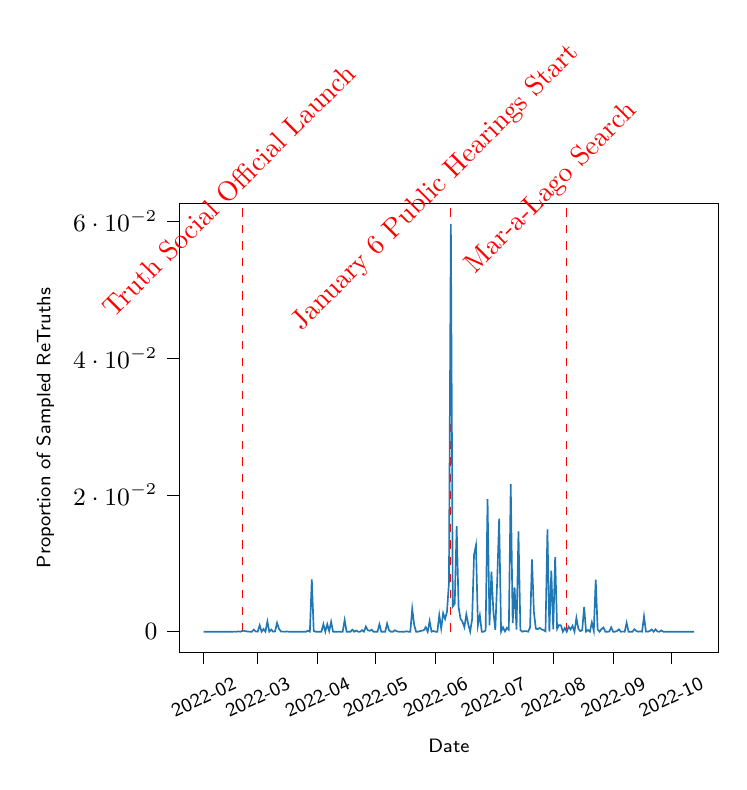
\begin{tikzpicture}

\definecolor{darkgray176}{RGB}{176,176,176}
\definecolor{steelblue31119180}{RGB}{31,119,180}

\begin{axis}[
tick align=outside,
tick pos=left,
xlabel={Date},
xticklabel style={rotate=25.0},
ylabel={Proportion of Sampled ReTruths},
clip=false,
x grid style={darkgray176},
xmin=19011.3, xmax=19290.7,
xtick style={color=black},
xtick={19024,19052,19083,19113,19144,19174,19205,19236,19266},
xticklabels={2022-02,2022-03,2022-04,2022-05,2022-06,2022-07,2022-08,2022-09,2022-10},
y grid style={darkgray176},
ymin=-0.00297829783463826, ymax=0.0625442545274035,
ytick style={color=black}
]

\addplot +[red, dashed, mark=none] coordinates
{(19044, 0) (19044, 0.0625442545274035)} node[above, rotate=45] {Truth Social Official Launch};
\addplot +[red, dashed, mark=none] coordinates
{(19152, 0) (19152, 0.0625442545274035)} node[above, rotate=45] {January 6 Public Hearings Start};
\addplot +[red, dashed, mark=none] coordinates
{(19212, 0) (19212, 0.0625442545274035)} node[above, rotate=45] {Mar-a-Lago Search};
% \addplot +[red, dashed, mark=none] coordinates
% {(19131, 0) (19131, 0.0625442545274035)} node[above, rotate=45] {Jan 6 Committee requests testimony from Rep. Barry Loudermilk};

% Jan 6 Committee requests testimony from Rep. Barry Loudermilk: 19131
\addplot [semithick, steelblue31119180]
table {%
19024 0
19025 0
19026 0
19027 0
19028 0
19029 0
19030 0
19031 0
19032 0
19033 0
19034 0
19035 0
19036 0
19037 0
19038 0
19039 0
19040 8.49589830166993e-06
19041 0
19042 4.73342905378753e-05
19043 0
19044 0.000127438474525049
19045 0.000121369975738142
19046 5.58301888395453e-05
19047 1.57780968459584e-05
19048 0
19049 0
19050 0.000309493438132262
19051 2.42739951476284e-05
19052 7.28219854428851e-06
19053 0.000947899510514888
19054 3.64109927214426e-06
19055 0.000387170222604672
19056 0
19057 0.00150498769915296
19058 1.57780968459584e-05
19059 0.000315561936919169
19060 0
19061 5.09753898100196e-05
19062 0.0012865217428243
19063 0.000435718212899929
19064 2.67013946623912e-05
19065 1.57780968459584e-05
19066 0
19067 3.03424939345355e-05
19068 0
19069 0
19070 0
19071 3.64109927214426e-06
19072 0
19073 0
19074 0
19075 0
19076 0
19077 0
19078 0.00015413986918744
19079 1.21369975738142e-06
19080 0.00765237697028984
19081 0.000101950779620039
19082 0
19083 0
19084 0
19085 0
19086 0.00110203937970233
19087 0
19088 0.00109354348140066
19089 9.34548813183692e-05
19090 0.0014564397088577
19091 4.85479902952567e-06
19092 0
19093 0
19094 6.06849878690709e-06
19095 0
19096 0
19097 0.00169917966033399
19098 0
19099 0
19100 0
19101 0.000287646842499396
19102 0
19103 0.000177200164577687
19104 0
19105 0
19106 0.000224534455115562
19107 0
19108 0.000747639050546954
19109 0.000218465956328655
19110 0.000127438474525049
19111 0.000276723544682963
19112 0
19113 0
19114 0
19115 0.00108626128285637
19116 0
19117 0
19118 0
19119 0.0011821435636895
19120 0.000180841263849831
19121 0
19122 0
19123 0.000211183757784367
19124 5.94712881116895e-05
19125 0
19126 6.06849878690709e-06
19127 0
19128 0
19129 5.94712881116895e-05
19130 0
19131 0
19132 0.00334981133037272
19133 0.00100130229983967
19134 0
19135 0
19136 9.34548813183692e-05
19137 0.000143216571371007
19138 0.000223320755358181
19139 0.000665107467045017
19140 0
19141 0.00155110828993345
19142 0
19143 0.000110446677921709
19144 0
19145 0
19146 0.00242133101597593
19147 0.00047941140416566
19148 0.00270048196017366
19149 0.00186667022685262
19150 0.00291045201820064
19151 0.00713776827316012
19152 0.0595659566927653
19153 0.00369450206146904
19154 0.00409623668116229
19155 0.015439474613649
19156 0.00361075677820972
19157 0.00187516612515429
19158 0.00148314110352009
19159 0.000655397868985966
19160 0.00253056399414026
19161 0.00108868868237113
19162 1.69917966033399e-05
19163 0.00180841263849831
19164 0.0112449282521388
19165 0.0126431103726422
19166 0.000941831011727981
19167 0.00240919401840212
19168 0
19169 0
19170 0.000180841263849831
19171 0.0193585111302336
19172 0.000921198115852497
19173 0.00878111774465456
19174 0.00301847129660759
19175 0.000276723544682963
19176 0.00747639050546954
19177 0.0165111714994168
19178 0
19179 0.000646901970684296
19180 3.7624692478824e-05
19181 0.00057286628548403
19182 0.000287646842499396
19183 0.0215686583884252
19184 0.00127317104549311
19185 0.00647751560514463
19186 0.000300997539830592
19187 0.0146432875728068
19188 0.000234244053174614
19189 0
19190 9.22411815609878e-05
19191 8.49589830166993e-05
19192 0
19193 0.000610490977962853
19194 0.010557974189461
19195 0.0028546218293611
19196 0.000438145612414692
19197 0.000372605825516096
19198 0.00055587448888069
19199 0.000344690731096323
19200 0.000224534455115562
19201 5.94712881116895e-05
19202 0.0149418577131226
19203 0
19204 0.00893889871311415
19205 0.000343477031338941
19206 0.0109014512207999
19207 0.000415085317024445
19208 0.000970959805905135
19209 0.000930907713911548
19210 0
19211 0.000540096392034731
19212 0
19213 0.000730647253943614
19214 0.000328912634250364
19215 0.000852017229681756
19216 3.64109927214426e-06
19217 0.00200867309846625
19218 0.000447855210473743
19219 7.88904842297922e-05
19220 0.000217252256571274
19221 0.00361925267651139
19222 4.85479902952567e-06
19223 0.000256090648807479
19224 8.49589830166993e-06
19225 0.00135934372826719
19226 0.000144430271128389
19227 0.00762446187587007
19228 0.000337408532552034
19229 0
19230 0.000395666120906342
19231 0.000616559476749761
19232 0
19233 0
19234 1.33506973311956e-05
19235 0.00064204717165477
19236 0
19237 0
19238 0.000101950779620039
19239 0.000343477031338941
19240 0
19241 1.69917966033399e-05
19242 0
19243 0.00129865874039812
19244 0
19245 0
19246 0
19247 0.000361682527699663
19248 0.000116515176708616
19249 0
19250 4.00520919935868e-05
19251 0
19252 0.00224534455115562
19253 3.03424939345355e-05
19254 1.21369975738142e-06
19255 0.000104378179134802
19256 0.000321630435706076
19257 0
19258 0.000339835932066797
19259 1.82054963607213e-05
19260 0
19261 0.000184482363121976
19262 0
19263 0
19264 0
19265 0
19266 0
19267 0
19268 0
19269 0
19270 0
19271 0
19272 0
19273 0
19274 0
19275 0
19276 1.21369975738142e-06
19277 0
19278 0
};
\end{axis}

\end{tikzpicture}

    \caption{A plot showing the proportion of ReTruths related to January 6 (using keywords "Jan 6", "January 6", "Jan six", and "January 6").}
    \label{fig:daily_truth}
\end{figure}
\begin{figure}
    \centering
    % This file was created with tikzplotlib v0.10.1.
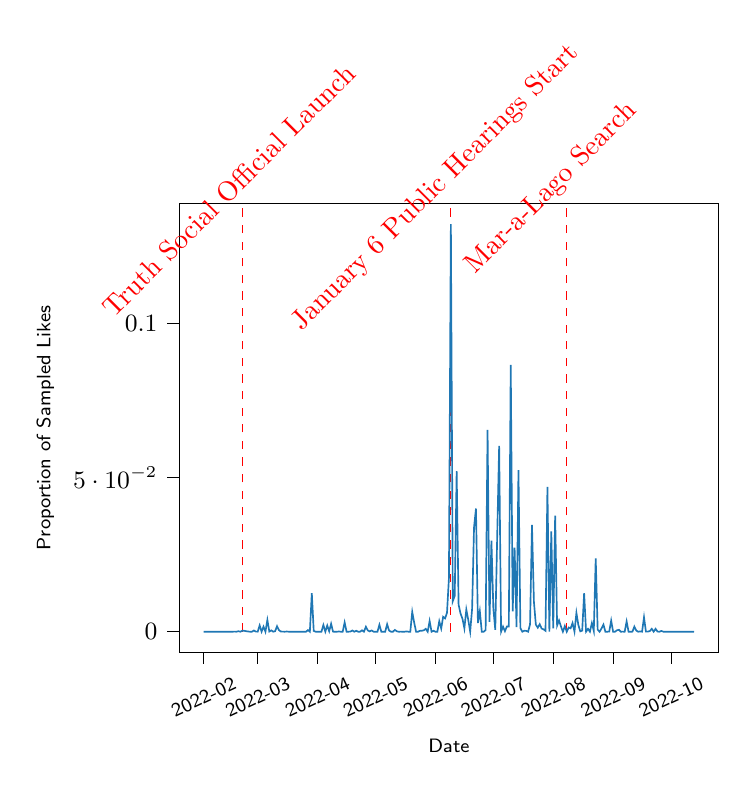
\begin{tikzpicture}

\definecolor{darkgray176}{RGB}{176,176,176}
\definecolor{steelblue31119180}{RGB}{31,119,180}

\begin{axis}[
tick align=outside,
xlabel={Date},
xticklabel style={rotate=25.0},
ylabel={Proportion of Sampled Likes},
clip=false,
tick pos=left,
x grid style={darkgray176},
xmin=19011.3, xmax=19290.7,
xtick style={color=black},
xtick={19024,19052,19083,19113,19144,19174,19205,19236,19266},
xticklabels={2022-02,2022-03,2022-04,2022-05,2022-06,2022-07,2022-08,2022-09,2022-10},
y grid style={darkgray176},
ymin=-0.00660944476877199, ymax=0.138798340144212,
ytick style={color=black}
]

\addplot +[red, dashed, mark=none] coordinates
{(19044, 0) (19044, 0.138798340144212)} node[above, rotate=45] {Truth Social Official Launch};
\addplot +[red, dashed, mark=none] coordinates
{(19152, 0) (19152, 0.138798340144212)} node[above, rotate=45] {January 6 Public Hearings Start};
\addplot +[red, dashed, mark=none] coordinates
{(19212, 0) (19212, 0.138798340144212)} node[above, rotate=45] {Mar-a-Lago Search};
% \addplot +[red, dashed, mark=none] coordinates
% {(19273, 0) (19273, 0.138798340144212)} node[above, rotate=45] {Jan 6 Committee subpoenas Trump};
\addplot [semithick, steelblue31119180]
table {%
19024 0
19025 0
19026 0
19027 0
19028 0
19029 0
19030 0
19031 0
19032 0
19033 0
19034 0
19035 0
19036 0
19037 0
19038 0
19039 7.28219854428851e-06
19040 2.3060295390247e-05
19041 4.85479902952567e-06
19042 0.000158994668216966
19043 0
19044 0.000326485234735602
19045 0.000286433142742015
19046 0.000168704266276017
19047 7.16082856855037e-05
19048 0
19049 0
19050 0.000400520919935868
19051 4.00520919935868e-05
19052 1.09232978164328e-05
19053 0.00206086218803365
19054 7.28219854428851e-06
19055 0.00163849467246492
19056 1.21369975738142e-06
19057 0.00382436793550885
19058 5.34027893247824e-05
19059 0.000434504513142548
19060 6.06849878690709e-06
19061 0.000158994668216966
19062 0.00178413864335069
19063 0.000490334701982093
19064 5.34027893247824e-05
19065 3.03424939345355e-05
19066 0
19067 5.70438885969267e-05
19068 4.85479902952567e-06
19069 1.21369975738142e-06
19070 0
19071 1.09232978164328e-05
19072 0
19073 0
19074 0
19075 3.64109927214426e-06
19076 1.21369975738142e-06
19077 0
19078 0.000520677195916629
19079 4.85479902952567e-06
19080 0.012512030798845
19081 0.000259731748079624
19082 1.21369975738142e-06
19083 0
19084 0
19085 3.64109927214426e-06
19086 0.00217252256571274
19087 6.06849878690709e-06
19088 0.00201474159725315
19089 0.000168704266276017
19090 0.00254876949050098
19091 1.69917966033399e-05
19092 0
19093 0
19094 6.43260871412152e-05
19095 2.42739951476284e-06
19096 3.64109927214426e-06
19097 0.00302211239587973
19098 2.42739951476284e-06
19099 0
19100 6.31123873838338e-05
19101 0.000396879820663724
19102 0
19103 0.000328912634250364
19104 9.70959805905135e-06
19105 1.21369975738142e-05
19106 0.000452710009503269
19107 0
19108 0.00159965628022871
19109 0.000406589418722775
19110 0.000117728876465998
19111 0.000405375718965394
19112 6.06849878690709e-06
19113 7.28219854428851e-06
19114 0
19115 0.00225384044945729
19116 2.42739951476284e-06
19117 2.42739951476284e-06
19118 0
19119 0.00243225431379236
19120 0.000373819525273477
19121 0
19122 7.28219854428851e-06
19123 0.000594712881116895
19124 0.000139575472098863
19125 0
19126 1.69917966033399e-05
19127 6.06849878690709e-06
19128 1.21369975738142e-06
19129 9.34548813183692e-05
19130 0
19131 2.42739951476284e-06
19132 0.00644595941145271
19133 0.00298084660412876
19134 0
19135 4.85479902952567e-06
19136 0.000288860542256778
19137 0.000302211239587973
19138 0.000483052503437805
19139 0.000936976212698455
19140 4.85479902952567e-06
19141 0.00348453200344205
19142 0
19143 0.000300997539830592
19144 2.42739951476284e-06
19145 6.06849878690709e-06
19146 0.0034032141196975
19147 0.00103649959280373
19148 0.00483780723292233
19149 0.00431834373676309
19150 0.00612554267550402
19151 0.0173959586225479
19152 0.13218889537544
19153 0.0099219955165931
19154 0.0116260299759566
19155 0.0520919935868105
19156 0.00876655334756599
19157 0.00590829041893275
19158 0.00420546965932661
19159 0.00106077358795136
19160 0.00720573545957348
19161 0.00387898442459101
19162 2.06328958754841e-05
19163 0.0074132781180857
19164 0.0338998479234204
19165 0.0399452864149372
19166 0.00283277523372823
19167 0.00667898976486995
19168 1.21369975738142e-06
19169 0
19170 0.000535241593005206
19171 0.0654621101141242
19172 0.00316411526749336
19173 0.029523246598303
19174 0.00750187820037455
19175 0.000589858082087369
19176 0.0313158811399554
19177 0.0602516970556858
19178 0
19179 0.0016591275683404
19180 0.00014564397088577
19181 0.00170524815912089
19182 0.00167733306470112
19183 0.086507663907118
19184 0.00663165547433207
19185 0.0272645513498162
19186 0.00147707260473319
19187 0.0523808541290673
19188 0.00117971616417474
19189 2.42739951476284e-06
19190 0.000311920837647025
19191 0.000258518048322242
19192 0
19193 0.00240676661888735
19194 0.0346135033807607
19195 0.00972416245613992
19196 0.00229389254145088
19197 0.00130715463869979
19198 0.00242861321452022
19199 0.00102921739425944
19200 0.000742784251517428
19201 0.000298570140315829
19202 0.046938624416969
19203 0
19204 0.0325332219966089
19205 0.00109839828043018
19206 0.037685377466693
19207 0.00199774980064981
19208 0.00367386916559355
19209 0.00168947006227493
19210 0
19211 0.00184482363121976
19212 3.64109927214426e-06
19213 0.00135934372826719
19214 0.00110446677921709
19215 0.00281214233785275
19216 9.70959805905135e-06
19217 0.00610855087890068
19218 0.00219558286110299
19219 0.000126224774767668
19220 0.000349545530125849
19221 0.0125071759998155
19222 1.4564397088577e-05
19223 0.000924839215124641
19224 1.09232978164328e-05
19225 0.00279272314173464
19226 0.000241526251718902
19227 0.0238042933415218
19228 0.000677244464618831
19229 1.21369975738142e-06
19230 0.00106926948625303
19231 0.00229874734048041
19232 2.42739951476284e-06
19233 0
19234 5.2189089567401e-05
19235 0.00361682527699663
19236 0
19237 2.42739951476284e-06
19238 0.000464847007077083
19239 0.000629910174080956
19240 2.42739951476284e-06
19241 2.06328958754841e-05
19242 0
19243 0.00334981133037272
19244 4.85479902952567e-06
19245 0
19246 1.33506973311956e-05
19247 0.00166034126809778
19248 0.000365323626971807
19249 0
19250 9.70959805905135e-05
19251 3.64109927214426e-06
19252 0.00466910296664632
19253 2.3060295390247e-05
19254 3.03424939345355e-05
19255 0.000212397457541748
19256 0.000944258411242744
19257 2.42739951476284e-06
19258 0.000934548813183692
19259 3.27698934492983e-05
19260 0
19261 0.000259731748079624
19262 1.21369975738142e-05
19263 0
19264 0
19265 6.06849878690709e-06
19266 0
19267 0
19268 0
19269 8.49589830166993e-06
19270 1.21369975738142e-06
19271 1.21369975738142e-06
19272 0
19273 0
19274 0
19275 2.42739951476284e-06
19276 3.64109927214426e-06
19277 0
19278 1.57780968459584e-05
};
\end{axis}

\end{tikzpicture}

    \caption{A plot showing the proportion of likes related to January 6 (using keywords "Jan 6", "January 6", "Jan Six", and "January Six").}
    \label{fig:daily_truth}
\end{figure}

\begin{figure}
    \centering
    % This file was created with tikzplotlib v0.10.1.
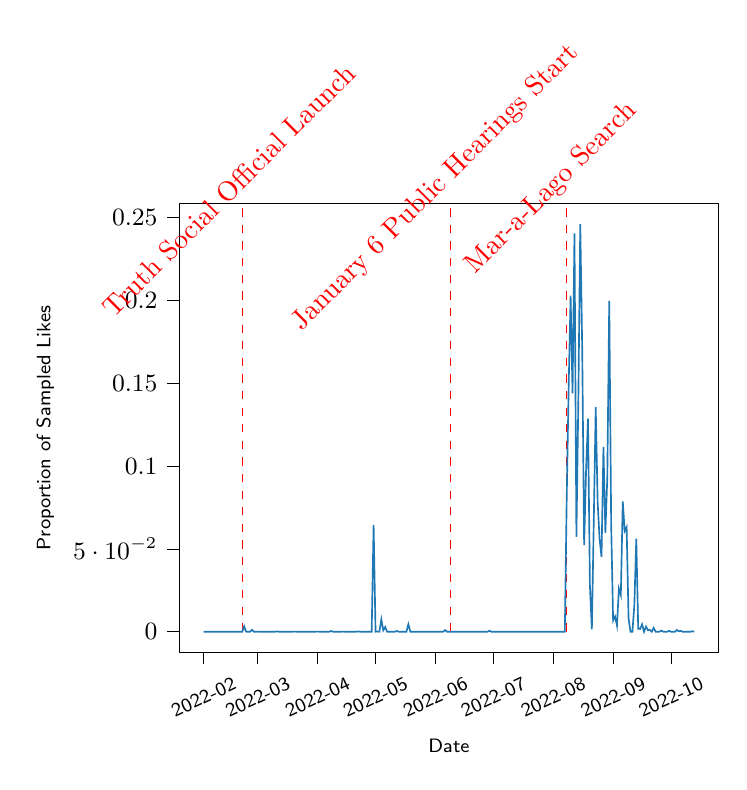
\begin{tikzpicture}

\definecolor{darkgray176}{RGB}{176,176,176}
\definecolor{steelblue31119180}{RGB}{31,119,180}

\begin{axis}[
tick align=outside,
tick pos=left,
x grid style={darkgray176},
xmin=19011.3, xmax=19290.7,
xlabel={Date},
xticklabel style={rotate=25.0},
ylabel={Proportion of Sampled Likes},
clip=false,
xtick style={color=black},
xtick={19024,19052,19083,19113,19144,19174,19205,19236,19266},
xticklabels={2022-02,2022-03,2022-04,2022-05,2022-06,2022-07,2022-08,2022-09,2022-10},
y grid style={darkgray176},
ymin=-0.0123041240304056, ymax=0.258386604638518,
ytick style={color=black}
]

\addplot +[red, dashed, mark=none] coordinates
{(19044, 0) (19044, 0.258386604638518)} node[above, rotate=45] {Truth Social Official Launch};
\addplot +[red, dashed, mark=none] coordinates
{(19152, 0) (19152, 0.258386604638518)} node[above, rotate=45] {January 6 Public Hearings Start};
\addplot +[red, dashed, mark=none] coordinates
{(19212, 0) (19212, 0.258386604638518)} node[above, rotate=45] {Mar-a-Lago Search};

\addplot [semithick, steelblue31119180]
table {%
19024 0
19025 0
19026 0
19027 0
19028 0
19029 0
19030 0
19031 0
19032 0
19033 0
19034 0
19035 0
19036 0
19037 0
19038 0
19039 0
19040 0
19041 1.21369975738142e-06
19042 0
19043 0
19044 0
19045 0.00327698934492983
19046 3.03424939345355e-05
19047 0
19048 1.21369975738142e-05
19049 0.00117000656611569
19050 0
19051 0
19052 3.15561936919169e-05
19053 0
19054 0
19055 0
19056 4.85479902952567e-06
19057 0
19058 0
19059 0
19060 0
19061 0
19062 0.000175986464820306
19063 0
19064 0
19065 0
19066 0
19067 0
19068 0
19069 0
19070 0
19071 7.40356852002665e-05
19072 0
19073 0
19074 0
19075 0
19076 0
19077 0
19078 0
19079 0
19080 0
19081 0
19082 9.70959805905135e-06
19083 6.6753486655978e-05
19084 0
19085 3.64109927214426e-06
19086 0
19087 0
19088 0
19089 0
19090 0.000421153815811352
19091 0
19092 0
19093 0
19094 0
19095 0
19096 4.49068910231125e-05
19097 0
19098 0
19099 0
19100 0
19101 0
19102 0
19103 0
19104 0.00018812346239412
19105 0
19106 0
19107 0
19108 0
19109 0
19110 0
19111 0
19112 0.0644474571169533
19113 0
19114 0.000117728876465998
19115 0
19116 0.00746182610838096
19117 0.000805896638901262
19118 0.00284005743227252
19119 1.21369975738142e-06
19120 0
19121 0
19122 0
19123 2.42739951476284e-06
19124 0.000411444217752301
19125 0
19126 0
19127 0
19128 0
19129 0
19130 0.00452710009503269
19131 0
19132 0
19133 0
19134 0
19135 1.21369975738142e-06
19136 1.21369975738142e-06
19137 0
19138 0
19139 0
19140 0
19141 0
19142 0
19143 0
19144 0
19145 0
19146 0
19147 0
19148 0
19149 0.000981883103721568
19150 0
19151 0
19152 0
19153 0
19154 0
19155 0
19156 0
19157 0
19158 0
19159 0
19160 3.64109927214426e-06
19161 0
19162 0
19163 0
19164 0
19165 0
19166 0
19167 0
19168 0
19169 0
19170 0
19171 0
19172 0.000592285481602132
19173 0
19174 0
19175 0
19176 0
19177 0
19178 0
19179 0
19180 0
19181 0
19182 2.42739951476284e-06
19183 0
19184 0
19185 0
19186 2.06328958754841e-05
19187 0
19188 0
19189 0
19190 0
19191 0
19192 0
19193 0
19194 0
19195 0
19196 0
19197 0
19198 0
19199 0
19200 0
19201 0
19202 0
19203 0
19204 0
19205 0
19206 0
19207 0
19208 0
19209 0
19210 0
19211 0
19212 0.0823944354293524
19213 0.148553209204213
19214 0.202851708949943
19215 0.143846481545088
19216 0.240490965825856
19217 0.0573278943401539
19218 0.139497795314391
19219 0.246082480608112
19220 0.171291874158754
19221 0.0522412786569684
19222 0.0970146627067689
19223 0.128697081173453
19224 0.0276444393738766
19225 0.00144915751031341
19226 0.0671977007671796
19227 0.135571476599262
19228 0.0782193082639603
19229 0.0559054382245029
19230 0.0452503680544514
19231 0.111547503601654
19232 0.0597395157580708
19233 0.0934463854200676
19234 0.199731286873716
19235 0.0649717754121421
19236 0.00681128303842452
19237 0.00918406606410519
19238 0.0036447403714164
19239 0.0260459967934052
19240 0.0221718671678438
19241 0.0787108566656998
19242 0.060761450953786
19243 0.063160935374129
19244 0.00794487861181876
19245 0
19246 1.21369975738142e-06
19247 0.016212601359101
19248 0.056185802868458
19249 0.00175500984917353
19250 0.00166155496785516
19251 0.00451860419673102
19252 2.42739951476284e-06
19253 0.0030827973837488
19254 0.000947899510514888
19255 0.0011433051714533
19256 9.70959805905135e-06
19257 0.00231695283684113
19258 1.69917966033399e-05
19259 0
19260 2.42739951476284e-06
19261 0.000668748566317162
19262 6.06849878690709e-06
19263 0
19264 0
19265 0.000518249796401866
19266 0
19267 0
19268 0
19269 0.00102072149595777
19270 0.000259731748079624
19271 0.00051339499737234
19272 0
19273 1.21369975738142e-06
19274 0
19275 0
19276 3.64109927214426e-06
19277 0.000282792043469871
19278 0
};
\end{axis}

\end{tikzpicture}

    \caption{A plot showing the proportion of likes related to the Mar-a-Lago Raid (using keywords "Mar-a-Lago" and "Mar a Lago".}
    \label{fig:daily_truth}
\end{figure}

\begin{figure}
    \centering
    % This file was created with tikzplotlib v0.10.1.
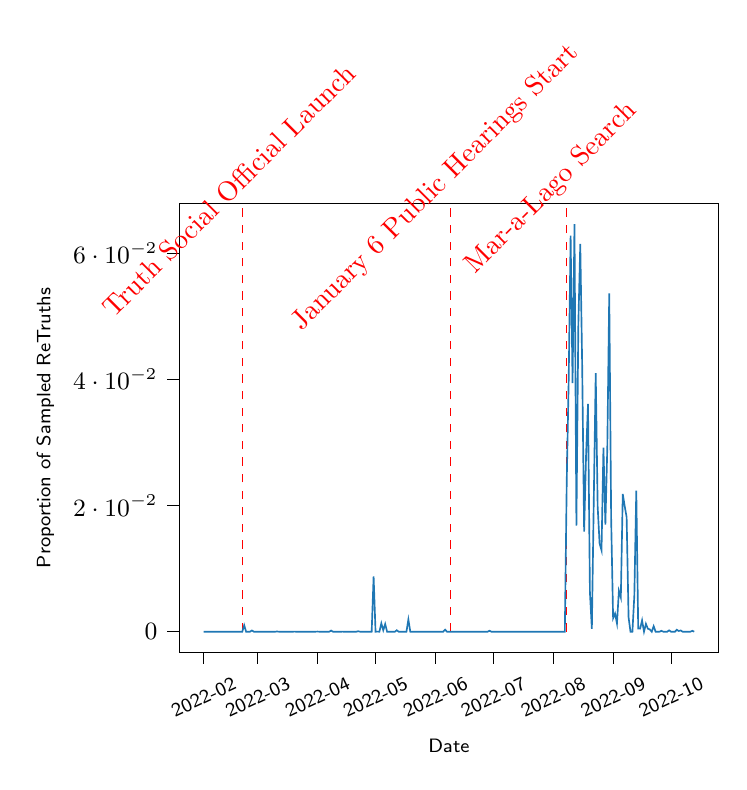
\begin{tikzpicture}

\definecolor{darkgray176}{RGB}{176,176,176}
\definecolor{steelblue31119180}{RGB}{31,119,180}

\begin{axis}[
tick align=outside,
tick pos=left,
x grid style={darkgray176},
xmin=19011.3, xmax=19290.7,
xtick style={color=black},
xtick={19024,19052,19083,19113,19144,19174,19205,19236,19266},
xlabel={Date},
xticklabel style={rotate=25.0},
ylabel={Proportion of Sampled ReTruths},
clip=false,
xticklabels={2022-02,2022-03,2022-04,2022-05,2022-06,2022-07,2022-08,2022-09,2022-10},
y grid style={darkgray176},
ymin=-0.00322825929967097, ymax=0.0677934452930903,
ytick style={color=black}
],
\addplot +[red, dashed, mark=none] coordinates
{(19044, 0) (19044, 0.0677934452930903)} node[above, rotate=45] {Truth Social Official Launch};
\addplot +[red, dashed, mark=none] coordinates
{(19152, 0) (19152, 0.0677934452930903)} node[above, rotate=45] {January 6 Public Hearings Start};
\addplot +[red, dashed, mark=none] coordinates
{(19212, 0) (19212, 0.0677934452930903)} node[above, rotate=45] {Mar-a-Lago Search};

\addplot [semithick, steelblue31119180]
table {%
19024 0
19025 0
19026 0
19027 0
19028 0
19029 0
19030 0
19031 0
19032 0
19033 0
19034 0
19035 0
19036 0
19037 0
19038 0
19039 0
19040 0
19041 0
19042 0
19043 0
19044 0
19045 0.00102921739425944
19046 0
19047 0
19048 0
19049 0.000199046760210553
19050 0
19051 0
19052 3.64109927214426e-06
19053 0
19054 0
19055 0
19056 1.21369975738142e-06
19057 0
19058 0
19059 0
19060 0
19061 0
19062 4.00520919935868e-05
19063 0
19064 0
19065 0
19066 0
19067 0
19068 0
19069 0
19070 0
19071 1.57780968459584e-05
19072 0
19073 0
19074 0
19075 0
19076 0
19077 0
19078 0
19079 0
19080 0
19081 0
19082 7.28219854428851e-06
19083 2.42739951476284e-05
19084 0
19085 0
19086 0
19087 0
19088 0
19089 0
19090 0.00017962756409245
19091 0
19092 0
19093 0
19094 0
19095 0
19096 1.09232978164328e-05
19097 0
19098 0
19099 0
19100 0
19101 0
19102 0
19103 0
19104 7.64630847150294e-05
19105 0
19106 0
19107 0
19108 0
19109 0
19110 0
19111 0
19112 0.00876291224829384
19113 0
19114 1.94191961181027e-05
19115 0
19116 0.00132900123433265
19117 0.000231816653659851
19118 0.00122098195592571
19119 0
19120 0
19121 0
19122 0
19123 0
19124 0.000231816653659851
19125 0
19126 0
19127 0
19128 0
19129 0
19130 0.00194191961181027
19131 0
19132 0
19133 0
19134 0
19135 0
19136 0
19137 0
19138 0
19139 0
19140 0
19141 0
19142 0
19143 0
19144 0
19145 0
19146 0
19147 0
19148 0
19149 0.000324057835220839
19150 0
19151 0
19152 0
19153 0
19154 0
19155 0
19156 0
19157 0
19158 0
19159 0
19160 0
19161 0
19162 0
19163 0
19164 0
19165 0
19166 0
19167 0
19168 0
19169 0
19170 0
19171 0
19172 0.000152926169430059
19173 0
19174 0
19175 0
19176 0
19177 0
19178 0
19179 0
19180 0
19181 0
19182 0
19183 0
19184 0
19185 0
19186 1.21369975738142e-06
19187 0
19188 0
19189 0
19190 0
19191 0
19192 0
19193 0
19194 0
19195 0
19196 0
19197 0
19198 0
19199 0
19200 0
19201 0
19202 0
19203 0
19204 0
19205 0
19206 0
19207 0
19208 0
19209 0
19210 0
19211 0
19212 0.0239657154092535
19213 0.0397802232479334
19214 0.0627628418537079
19215 0.0393979078243582
19216 0.0645651859934193
19217 0.0168133827390048
19218 0.0486402314768177
19219 0.0614544735152507
19220 0.0419163348209247
19221 0.0158666969282473
19222 0.0279223766183169
19223 0.0360857211864643
19224 0.00619108246240262
19225 0.000450282609988506
19226 0.0210504085920233
19227 0.0409465887147769
19228 0.0198524869314879
19229 0.0139842486045487
19230 0.0129089106195088
19231 0.0291785558672067
19232 0.0169711637074644
19233 0.0292076846613838
19234 0.0535787757896027
19235 0.0177163753584966
19236 0.00214339377153558
19237 0.00288132322402349
19238 0.00130351353942764
19239 0.00649450740174797
19240 0.00542038311646542
19241 0.0218332449355343
19242 0.0198961801227536
19243 0.0181581620701834
19244 0.00230360213950993
19245 0
19246 0
19247 0.00577842454489293
19248 0.0223660591290248
19249 0.000496403200769
19250 0.000486693602709949
19251 0.0017962756409245
19252 0
19253 0.00123797375252905
19254 0.000481838803680423
19255 0.000360468827942281
19256 1.21369975738142e-06
19257 0.00088114602385891
19258 6.06849878690709e-06
19259 0
19260 1.21369975738142e-06
19261 0.00014564397088577
19262 1.21369975738142e-06
19263 0
19264 0
19265 0.00021361115729913
19266 0
19267 0
19268 0
19269 0.000311920837647025
19270 0.000110446677921709
19271 0.000201474159725315
19272 0
19273 0
19274 0
19275 0
19276 1.21369975738142e-06
19277 0.000143216571371007
19278 0
};
\end{axis}

\end{tikzpicture}

    \caption{A plot showing the proportion of ReTruths related to the Mar-a-Lago Raid (using keywords "Mar-a-Lago" and "Mar a Lago".}
    \label{fig:daily_truth}
\end{figure}
\fi

\section{Conclusion}
This paper presents a large dataset, which contains information of 454,000 users and over 823,000 posts including the complete history of the 65,536 most active users from the Truth Social platform. In addition, this dataset covers the ReTruths, quotes, text, media, and other information from the platform. We also perform a preliminary analysis of this dataset. 

Our preliminary analysis shows that a handful of external Web sites dominate Truth Social posts, with Rumble appearing most frequently. Moreover, a brief look at the most commonly linked Telegram channels finds that right-wing and Trump-focused Telegram channels appear most often. We also analyzed the temporal and structural nature of the posts and ReTruths in the dataset. We have uncovered several interesting findings and avenues for further study.





% number of Truths posted containing certain keywords, we were able
% Additionally, our analysis points to a relatively constant number of Truths posted per day, as well as a

% Additionally, our analysis illustrates how external events may have influenced behavior on Truth Social, specifically the U.S. January 6 Committee~\cite{broadwater_haberman} and the Mar-a-Lago Search. Finally, our analysis shows that posts on Truth Social have remained relatively constant after an initial spike at its launch.

Overall, Truth Social is an emerging alt-tech platform. Targeted at hard-right users disaffected from mainstream social media platforms and working as the main mouthpiece of former President Donald Trump, Truth Social's unique position in the information ecosystem cannot be overlooked. This dataset provides researchers a means to study the Truth Social platform, permitting research on both Truth Social itself and important socio-technical issues including the cultivation and spread of information and narratives.




\bibliography{citations}

\end{document}
